\documentclass[notes,11pt, aspectratio=169]{beamer}

\usepackage{pgfpages}
% These slides also contain speaker notes. You can print just the slides,
% just the notes, or both, depending on the setting below. Comment out the want
% you want.
\setbeameroption{hide notes} % Only slide
%\setbeameroption{show only notes} % Only notes
%\setbeameroption{show notes on second screen=right} % Both

\usepackage{helvet}
\usepackage[default]{lato}
\usepackage{array}
\usepackage{tgbonum}

\usepackage{tikz}
\usepackage{verbatim}
\setbeamertemplate{note page}{\pagecolor{yellow!5}\insertnote}
\usetikzlibrary{positioning}
\usetikzlibrary{snakes}
\usetikzlibrary{calc}
\usetikzlibrary{arrows}
\usetikzlibrary{decorations.markings}
\usetikzlibrary{shapes.misc}
\usetikzlibrary{matrix,shapes,arrows,fit,tikzmark}
\usepackage{amsmath}
\usepackage{mathpazo}
\usepackage{hyperref}
\usepackage{lipsum}
\usepackage{multimedia}
\usepackage{graphicx}
\usepackage{multirow}
\usepackage{graphicx}
\usepackage{dcolumn}
\usepackage{bbm}
\newcolumntype{d}[0]{D{.}{.}{5}}

\usepackage{changepage}
\usepackage{appendixnumberbeamer}
\newcommand{\beginbackup}{
   \newcounter{framenumbervorappendix}
   \setcounter{framenumbervorappendix}{\value{framenumber}}
   \setbeamertemplate{footline}
   {
     \leavevmode%
     \hline
     box{%
       \begin{beamercolorbox}[wd=\paperwidth,ht=2.25ex,dp=1ex,right]{footlinecolor}%
%         \insertframenumber  \hspace*{2ex} 
       \end{beamercolorbox}}%
     \vskip0pt%
   }
 }
\newcommand{\backupend}{
   \addtocounter{framenumbervorappendix}{-\value{framenumber}}
   \addtocounter{framenumber}{\value{framenumbervorappendix}} 
}


\usepackage{graphicx}
\usepackage[space]{grffile}
\usepackage{booktabs}
\newcommand\independent{\protect\mathpalette{\protect\independenT}{\perp}}
\def\independenT#1#2{\mathrel{\rlap{$#1#2$}\mkern2mu{#1#2}}}
\DeclareMathOperator{\Supp}{Supp}

% These are my colors -- there are many like them, but these ones are mine.
\definecolor{blue}{RGB}{0,114,178}
\definecolor{red}{RGB}{213,94,0}
\definecolor{yellow}{RGB}{240,228,66}
\definecolor{green}{RGB}{0,158,115}

\hypersetup{
  colorlinks=false,
  linkbordercolor = {white},
  linkcolor = {blue}
}
\usepackage{booktabs}
\usepackage{mathtools}
\usepackage{multirow}
\usepackage{bbm}
\usepackage{accents}

\newcommand\indep{\protect\mathpalette{\protect\independenT}{\perp}}
\DeclareMathOperator{\var}{var}
\DeclareMathOperator*{\argmin}{argmin}
\DeclarePairedDelimiter\indicatorfence{\{}{\}}
\DeclarePairedDelimiter\abs{\lvert}{\rvert}
\DeclarePairedDelimiter\norm{\lVert}{\rVert}
\DeclarePairedDelimiter\ip{\langle}{\rangle}
\newcommand\1{\operatorname{\mathbbm{1}}\indicatorfence}
\newcommand{\dbtilde}[1]{\accentset{\approx}{#1}}

%% I use a beige off white for my background
\definecolor{MyBackground}{RGB}{255,253,218}

%% Uncomment this if you want to change the background color to something else
%\setbeamercolor{background canvas}{bg=MyBackground}

%% Change the bg color to adjust your transition slide background color!
\newenvironment{transitionframe}{
  \setbeamercolor{background canvas}{bg=yellow}
  \begin{frame}}{
    \end{frame}
}

\setbeamercolor{frametitle}{fg=blue}
\setbeamercolor{title}{fg=black}
\setbeamertemplate{footline}[frame number]
\setbeamertemplate{navigation symbols}{} 
\setbeamertemplate{itemize items}{-}
\setbeamercolor{itemize item}{fg=blue}
\setbeamercolor{itemize subitem}{fg=blue}
\setbeamercolor{enumerate item}{fg=blue}
\setbeamercolor{enumerate subitem}{fg=blue}
\setbeamercolor{button}{bg=MyBackground,fg=blue,}



% If you like road maps, rather than having clutter at the top, have a roadmap show up at the end of each section 
% (and after your introduction)
% Uncomment this is if you want the roadmap!
% \AtBeginSection[]
% {
%    \begin{frame}
%        \frametitle{Roadmap of Talk}
%        \tableofcontents[currentsection]
%    \end{frame}
% }
\setbeamercolor{section in toc}{fg=blue}
\setbeamercolor{subsection in toc}{fg=red}
\setbeamersize{text margin left=1em,text margin right=1em} 

\newenvironment{wideitemize}{\itemize\addtolength{\itemsep}{10pt}}{\enditemize}

\usepackage{environ}
\NewEnviron{videoframe}[1]{
  \begin{frame}
    \vspace{-8pt}
    \begin{columns}[onlytextwidth, T] % align columns
      \begin{column}{.70\textwidth}
        \begin{minipage}[t][\textheight][t]
          {\dimexpr\textwidth}
          \vspace{8pt}
          \hspace{4pt} {\Large \sc \textcolor{blue}{#1}}
          \vspace{8pt}
          
          \BODY
        \end{minipage}
      \end{column}%
      \hfill%
      \begin{column}{.38\textwidth}
        \colorbox{green!20}{\begin{minipage}[t][1.2\textheight][t]
            {\dimexpr\textwidth}
            Face goes here
          \end{minipage}}
      \end{column}%
    \end{columns}
  \end{frame}
}

\title[]{\textcolor{blue}{Linear Regression II: Semiparametrics + Visualization}}
\author[PGP]{}
\institute[FRBNY]{\small{Paul Goldsmith-Pinkham}}
\date{\today}


\begin{document}

%%% TIKZ STUFF
\tikzset{   
        every picture/.style={remember picture,baseline},
        every node/.style={anchor=base,align=center,outer sep=1.5pt},
        every path/.style={thick},
        }
\newcommand\marktopleft[1]{%
    \tikz[overlay,remember picture] 
        \node (marker-#1-a) at (-.3em,.3em) {};%
}
\newcommand\markbottomright[2]{%
    \tikz[overlay,remember picture] 
        \node (marker-#1-b) at (0em,0em) {};%
}
\tikzstyle{every picture}+=[remember picture] 
\tikzstyle{mybox} =[draw=black, very thick, rectangle, inner sep=10pt, inner ysep=20pt]
\tikzstyle{fancytitle} =[draw=black,fill=red, text=white]
%%%% END TIKZ STUFF

% Title Slide
\begin{frame}
\maketitle

\end{frame}

% INTRO
\begin{frame}{Linear Regression: Why so Popular?}
\begin{columns}[T] % align columns
\begin{column}{.8\textwidth}
  \begin{wideitemize}
  \item Linear regression is incredibly popular as a tool. Why? 
  \item Many reasons:
    \begin{itemize}
    \item Fast (easy analytic solution and matrix inversion has gotten better)
    \item Efficient (under some settings, OLS is BLUE)
    \end{itemize}
  \item My view: linear regressions is
    \begin{enumerate}
    \item an intuitive summary of data relationships
    \item A good default -- many ``better'' options are only good in
      some settings, and linear regression is not bad in many
    \item Does a good job with many of the things we throw at our
      models (high dimensional fixed effects, lots of data)
    \end{enumerate}
  \item Today: how to stay in the world of linear regression as much
    as possible, improving our presentation
    \begin{itemize}
    \item As a side goal, we will do a discussion on good visualization practice
    \end{itemize}
  \end{wideitemize}
  \end{column}%
  \hfill%
  \begin{column}{.5\textwidth}
  \end{column}
\end{columns}
\end{frame}

\begin{frame}{General framework of causal relationships}
  \begin{wideitemize}
  \item Without any structure, we can describe our usual relationships
    as $Y_{i} = F(D_{i}, W_{i},\epsilon_{i})$
    \begin{itemize}
    \item $D_{i}$ is some causal variable we care about
    \item $W_{i}$ is controls / heterogeneity
    \item $\epsilon_{i}$ is unobservable noise
    \item Very unrestricted!
    \end{itemize}
  \item This function is very challenging to estimate with
    non-seperable $\epsilon_{i}$ and if the dimension of $D_{i}$ or
    $W_{i}$ is high
    \begin{itemize}
    \item Simpler: $Y_{i} = F(D_{i}, W_{i}) + \epsilon_{i}$
    \item What do we report from this? $E\left(\frac{\partial{F}}{\partial D_{i}} \middle| W_{i} = w\right)?$ $E\left(\frac{\partial{F}}{\partial D_{i}} \right)$?
    \end{itemize}
  \item What does a simple linear model get us to? $Y_{i} = D_{i}\tau + W_{i}\beta + \epsilon_{i}$
    \begin{itemize}
    \item Can be more complex! E.g.
      $Y_{i} = D_{i}\tau + W_{i}\beta_{1} + D_{i} \times
      W_{i}\beta_{2} + \epsilon_{i}$, etc.
    \item However, in this setting there is not a ``single'' number
      either
    \end{itemize}
  \end{wideitemize}
\end{frame}

\begin{frame}{Visualizing a relationship}
  \begin{columns}[T] % align columns
    \begin{column}{.5\textwidth}
      \begin{wideitemize}
  \item<1-> Intuitively, for many papers, we plot an outcome $Y_{i}$ and
    want to describe/assert a relationship/effect from $D_{i}$
  \item<1-> The line is a useful summary description of it, but the
    data already does a pretty good job. Why do we need the line?
  \item<2-> Well, sometimes we have a LOT more data and it's harder to
    see the relationship
  \item<2-> The line is an excellent summary
  \end{wideitemize}
  \end{column}%
  \hfill%
  \begin{column}{.5\textwidth}
    \only<1>{
      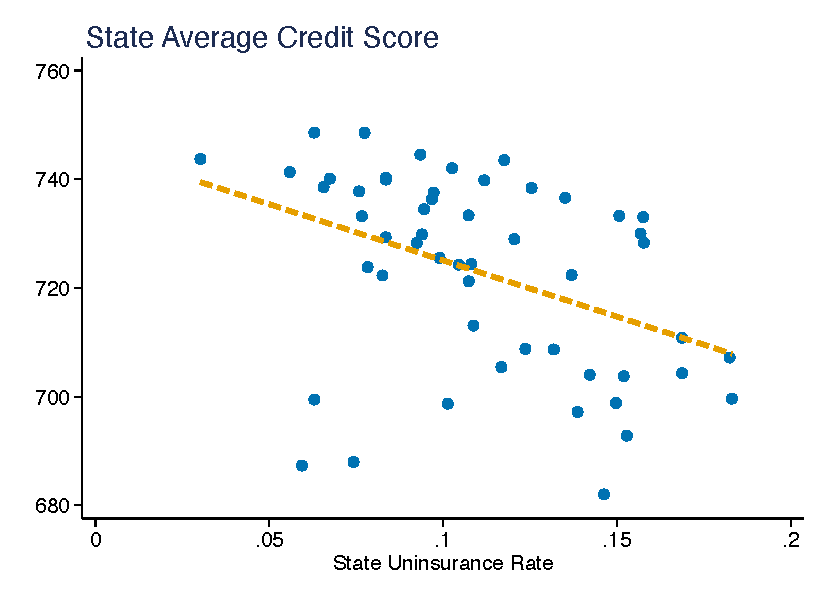
\includegraphics[width=\linewidth]{images/example_scatter1.pdf}
      }
    \only<2>{
      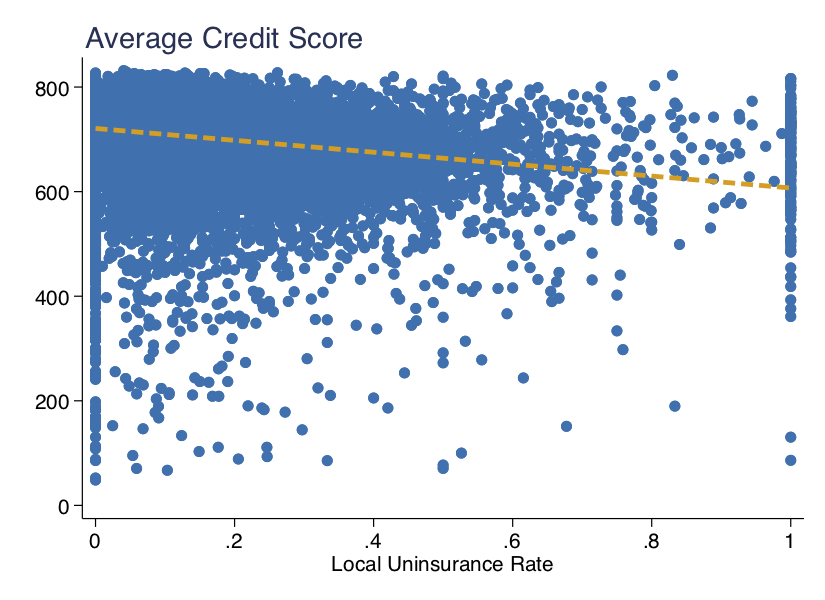
\includegraphics[width=\linewidth]{images/example_scatter2.png}
      }
  \end{column}
\end{columns}
\end{frame}

\begin{frame}{Visualizing a \emph{multivariate} relationship}
  \begin{wideitemize}
  \item What about controls? E.g. we have a causal estimand conditional on a set of covariates $W$
  \item First, an aside. Let $W$ be discrete -- e.g., we think the
    effect of $D$ is causal, but only conditional on fixed effects.
    \begin{itemize}
    \item How can we think about the OLS regression?
    \end{itemize}
  \item In the pscore setting, we would estimate
    $\tau(w) = E(Y|D_{i}=1, W=w) - E(Y | D_{i} = 0, W = w)$, and then
    aggregate this using the distribution of the $w$ (using IPW)
    \begin{itemize}
    \item With OLS, this is done for us automatically. How?
    \end{itemize}
  \item Recall in a regression, our setup is
    $$ Y_{i} = \tau D_{i} + \beta W_{i} + \epsilon_{i}$$
  \end{wideitemize}
\end{frame}

\begin{frame}{Residual Regression}
    $$ Y_{i} = \tau D_{i} + \beta W_{i} + \epsilon_{i}$$
  \begin{wideitemize}
  \item Consider the projection of $D_{i}$ and $Y_{i}$ onto $W_{i}$ 
    \begin{itemize}
      \item Note that if $W$ and $D$ are uncorrelated, we don't have to worry about controlling for it.
      \end{itemize}
    \item We define a projection matrix as $\mathbf{P}_{W} = \mathbf{W}_{n}(\mathbf{W}_{n}'\mathbf{W}_{n})^{-1}\mathbf{W}_{n}$
      \begin{itemize}
      \item Note that $\mathbf{P}_{W}\mathbf{W}_{n} = \mathbf{W}_{n}, \mathbf{P}_{W}\mathbf{P}_{W} = \mathbf{P}_{W}$
      \item Also note that $\mathbf{P}_{W}\mathbf{D}_{n}$ gives you
        the predicted values from a linear regression:
        $$D_{i} = \gamma W_{i} + u_{i}$$
      \end{itemize}
    \item Finally, denote $\mathbf{M}_{W} = \mathbf{I}_{n} - \mathbf{P}_{W}$ as the annhilator matrix
      \begin{itemize}
      \item This gives us the residual from the regression on $W_{i}$! (e.g. $u_{i}$ above).
      \end{itemize}
  \end{wideitemize}
\end{frame}

\begin{frame}{Frisch-Waugh-Lovell? More like Frisch-Wow-Lovell!}
  $$ Y_{i} = \tau D_{i} + \beta W_{i} + \epsilon_{i}$$
  \begin{wideitemize}
  \item Now if we transform $\mathbf{Y}_{n}^{*} = M_{W}\mathbf{Y}_{n}$ and $\mathbf{D}_{n}^{*} = M_{W}\mathbf{D}_{n}$, we can run
    $$ Y_{i}^{*} = \tau D^{*}_{i} +  \tilde{\epsilon}_{i}$$
    and get the right coefficient $\tau$! (This is the Frisch-Waugh-Lovell theorem)
  \item Consider $W$ as a discrete set of covariates. This will
    demean $D$ and $Y$ within each group. It is not too difficult to
    show that this regression estimate will get you
    \begin{equation}
      \tau = \frac{E(\sigma^{2}_{D}(W_{i})\tau(W_{i}))}{E(\sigma^{2}_{D}(W_{i}))}, \qquad \sigma^{2}_{D}(W_{i}) = E((D_{i} - E(D_{i}|W_{i}))^{2} | W_{i})
    \end{equation}
    Let's derive this, and show how it can fail more generally.
  \end{wideitemize}
\end{frame}

\begin{frame}
  \begin{itemize}
  \item To build intuition, consider both $W_{i}$ and $D_{i}$ binary. Then add another treatment arm.
  \item Consider regression
    \begin{equation*}
      Y_i=\alpha + D_{i}\beta+W_{i}\gamma +U_i,
    \end{equation*}
    with $D_{i},W_{i}\in\{0,1\}$. \alert{By definition}, $U_{i}$ mean-zero
    regression residual uncorrelated with $(D_{i},W_{i})$
  \item Stylized Project STAR example: $D_{i}$ is small classroom dummy, $Y_{i}$
    is avg test score of student $i$
    \begin{itemize}
    \item Randomization stratified: probability of assignment to small vs large
      classroom depends on school. $W_{i}$ denotes school FE
    \item Binary $W_{i}$: only 2 schools for simplicity
    \end{itemize}
  \end{itemize}
\end{frame}

\begin{frame}{Potential outcomes and key assumption}
  \begin{itemize}
  \item To characterize $\beta$, use potential outcomes notation $Y_{i}(d)$
    \begin{itemize}
    \item Individual treatment effect $\tau_{i1} = Y_{i}(1) - Y_{i}(0)$,
      conditional treatment effect $\tau_{1}(w) = E[\tau_{i1}\mid W_{i} = w]$
    \item Observed outcome $Y_{i} = Y_{i}(0) + \tau_{i1}D_{i}$
    \item Propensity score:
      $p_{1}(W_{i}) = \Pr(D_{i} = 1 \mid W_{i}) = E[D_{i} \mid W_{i}]$
    \end{itemize}
  \item Treatment (as good as) randomly assigned conditional on $W_{i}$:
    $\left(Y_i(0),Y_i(1)\right)\indep D_i\mid W_i$
  \item Random assignment assumption delivers key result from Angrist (1998):
    \begin{equation*}
      \beta=\phi\tau_{1}(0)+(1-\phi)\tau_{1}(1),\quad
      \phi= \frac{\var(D_i\mid W_i=0)\Pr(W_i=0)}{\sum_{w=0}^{1}
        \var(D_i\mid W_i=w)\Pr(W_i=w)},
    \end{equation*}
  \end{itemize}
\end{frame}

\begin{frame}{Derivation}
  \small
  \begin{equation*}
    \begin{split}
      \beta&\overset{(1)}{=}\frac{E[\tilde{D}_{i}Y_i]}{E[\tilde{D}_i^2]}
      % =\frac{E[\tilde{D}_i(Y_i(0)+\tau_{i1}D_i)]}{E[\tilde{D}_i^2]}
      =\frac{EE[\tilde{D}_{i}Y_i(0)\mid
        W_{i}]}{E[\tilde{D}_i^2]}+\frac{EE[\tilde{D}_{i} D_{i}\tau_{i1}\mid W_{i}]}{E[\tilde{D}_i^2]}\\
      & \overset{(2)}{=}\frac{E[\var(D_{i}\mid W_{i})\tau(W_i)]}{E[\var(D_{i}\mid W_{i})]}\\
      & =\phi\tau(0)+(1-\phi)\tau(1)\quad \phi= \frac{\var(D_i\mid
        W_i=0)\Pr(W_i=0)}{\sum_{w=0}^{1} \var(D_i\mid W_i=w)\Pr(W_i=w)},
    \end{split}
  \end{equation*}
  \begin{itemize}
  \item (1) follows from FWL theorem; $\tilde{D}_{i}$ residual from regressing
    $D_{i}$ on $W_{i}$.
  \item (2) follows by random assignment, and the fact that
    $E[\tilde{D}_{i}\mid W_{i}]=0$ (not just
    $\operatorname{corr}(\tilde{D}_{i},W_{i})=0$).
  \end{itemize}
\end{frame}

\begin{frame}{Key features of this estimator}
    \begin{equation*}
      \beta=\phi\tau(0)+(1-\phi)\tau(1),\quad
      \phi= \frac{\var(D_i\mid W_i=0)\Pr(W_i=0)}{\sum_{w=0}^{1}
        \var(D_i\mid W_i=w)\Pr(W_i=w)},
    \end{equation*}
  \begin{itemize}
  \item $\phi\in (0,1)$
  \item No need to estimate propensity score
  \item Puts larger weight on strata with higher variation in $D_{i}$
    \begin{itemize}
    \item $\neq$ ATE! (unless $\tau(w)$ constant or $p_{1}(w)$ constant
      across strata)
    \item May lead to unusual or ``unrepresentative'' estimand (Aronow and Samii (2016)
    \item But this sort of weighting necessary to avoid loss of identification
      under overlap failure (e.g. $p_{1}(0)=0$), or lack of precision under weak
      overlap ($p_{1}(0)$ close to $0$)
    \end{itemize}
  \end{itemize}
\end{frame}

\begin{frame}{Multiple treatments}

  \begin{itemize}
  \item Project STAR in fact had additional treatment arm in addition to small
    class ($D_{i}=1$): full-time teaching aide ($D_i=2$).
    \begin{equation*}
      Y_i=\alpha+  X_{i1}\beta_{1}+X_{i2}\beta_{2}+W_i\gamma +U_i,
    \end{equation*}
  \item General notation:
    \begin{itemize}
    \item $X_{i} = [X_{i1}, X_{i2}]'$, $X_{ij}=\1{D_{i}=j}$
    \item $Y_i=Y_i(0)+X_{i}'\tau_{i}$, where $\tau_{ik}=Y_{k}(k)-Y_{i}(0)$.
    \item Let $\tau_{k}(W_{i})=E[\tau_{ik}\mid W_{i}]$ and
      $p_{ok}(w)=E[X_{ik}\mid W_{i}=w]$.
    \end{itemize}
  \item Assignment still conditionally random,
    $\left(Y_i(0),Y_i(1),Y_i(2)\right)\perp {X}_i \mid W_i$
  \end{itemize}
\end{frame}

\begin{frame}{Causal interpretation of $\beta_{1}$}\label{slide:fwl_derivation}
  Again, due to FWL,
    \begin{equation*}
      \begin{split}
        \beta_{1}&=\frac{E[\dbtilde{X}_{i1}Y_i]}{E[\dbtilde{X}_{i1}^2]} =
        {\frac{E[\dbtilde{X}_{i1}Y_{i}(0)]}{E[\dbtilde{X}_{i1}^2]}}+
        \frac{E[\dbtilde{X}_{i1}X_{i1}\tau_{i1}]}{E[\dbtilde{X}_{i1}^2]}
        +\frac{E[\dbtilde{X}_{i1}X_{i2}\tau_{i2}]}{E[\dbtilde{X}_{i1}^2]}\\
        &= E[\lambda_{11}(W_{i})\tau_{1}(W_{i})]
        +E[\lambda_{12}(W_{i})\tau_{2}(W_{i})],
      \end{split}
     \end{equation*}
     where
     $ \lambda_{11}(W_{i})= \frac{E[\dbtilde{X}_{i1}X_{i1}\mid
       W_{i}]}{E[\dbtilde{X}_{i1}^2]} \geq 0$, and
     $\lambda_{12}(W_i) =\frac{E[\dbtilde{X}_{i1}X_{i2}\mid
       W_{i}]}{E[\dbtilde{X}_{i1}^2]} \neq 0$ in general.
  \begin{description}
  \item[Key point] $\dbtilde{X}_{i1}$ is residual from regressing $X_{i1}$ on
    $W_{i}$, constant, \alert{and} $X_{i2}$
    \begin{itemize}
    \item $\dbtilde{X}_{i1} \not= X_{i1} - E[X_{i1} \mid W_{i}, X_{i2}]$, since
      $X_{i2}$ \alert{depends non-linearly} on $X_{i1}$
    \item As a result, $\beta_{1}$ \alert{contaminated} by $\tau_{i2}$.
    \end{itemize}
  \end{description}
\end{frame}


\begin{frame}{Stylized Example: No overlap}
  \begin{itemize}
  \item Suppose only units in stratum $W_{i}=0$ receive treatment $2$. Let
    $n_{k}(w)=\sum_{i=1}^{N}\1{W_{i}=w,X_{i}=k}$.
  \item Then
    \begin{equation*}
      \hat{\beta}
      =
  \begin{pmatrix}
    \phi\hat{\tau}_{1}(0)+(1-\phi)\hat{\tau}_{1}(1)
    \\
    \frac{n_{1}(0)(1-\phi)}{n_{1}(0)+n_{0}(0)}
    \left[\hat{\tau}_{1}(1)-\hat{\tau}_{1}(0)\right]
    +\hat{\tau}_{2}(0)
  \end{pmatrix},
    \end{equation*}
    where
    $\phi=\frac{(1/n_{1}(0)+1/n_{0}(0))^{-1}}{
      \sum_{w=0}^{1}(1/n_{1}(w)+1/n_{0}(w))^{-1} }$.
  \item E.g., with equal-sized strata, $n_{0}(0)=n_{1}(0)=n_{2}(0)$, and
    $n_{0}(1)=n_{1}(1)$,
    \begin{equation*}
      \hat{\beta}
      =
      \begin{pmatrix}
        \frac{2}{5}\hat{\tau}_{1}(0)+\frac{3}{5}\hat{\tau}_{1}(1)
        \\
        \frac{3}{10}
        \left[\hat{\tau}_{1}(1)-\hat{\tau}_{1}(0)\right]
        +\hat{\tau}_{2}(0)
      \end{pmatrix}.
    \end{equation*}
  \end{itemize}
\end{frame}




\begin{frame}{Exploiting FWL for visualization}
  \begin{columns}[T] % align columns
    \begin{column}{.5\textwidth}
  \begin{wideitemize}
  \item<1-> Key point: we can still plot our line, but it would be nice to
    lay the line over data
  \item<1-> Why don't we exploit FWL and plot $Y^{*}$ and  $D^{*}$?
    \begin{itemize}
    \item Add in state fixed effects
    \end{itemize}
  \item<1-> Kind of hard to intuit b/c demeaned
  \item<2-> Easy solution -- add back the overall means
    \begin{itemize}
    \item Can you see an issue here?
    \end{itemize}
  \end{wideitemize}
  \end{column}%
  \hfill%
  \begin{column}{.5\textwidth}
    \only<1>{
      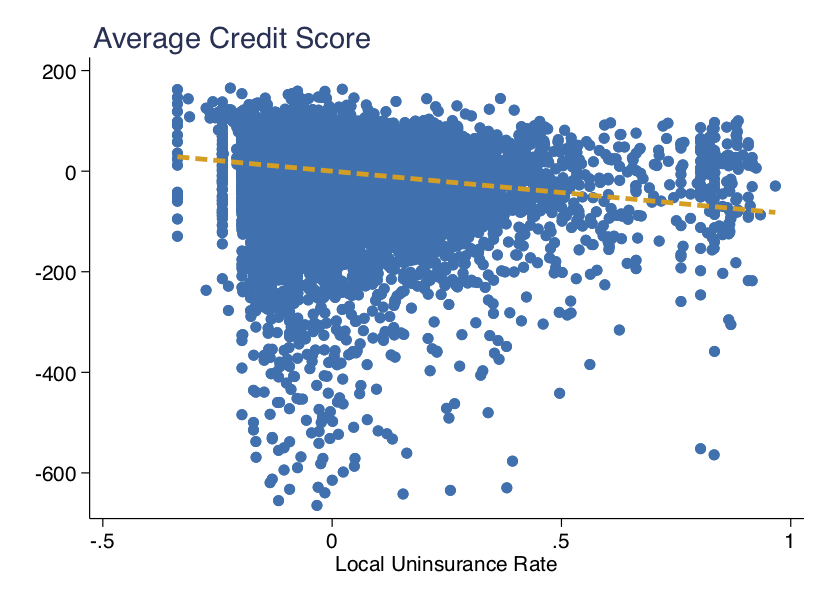
\includegraphics[width=\linewidth]{images/example_scatter3.png}
      }
    \only<2>{
      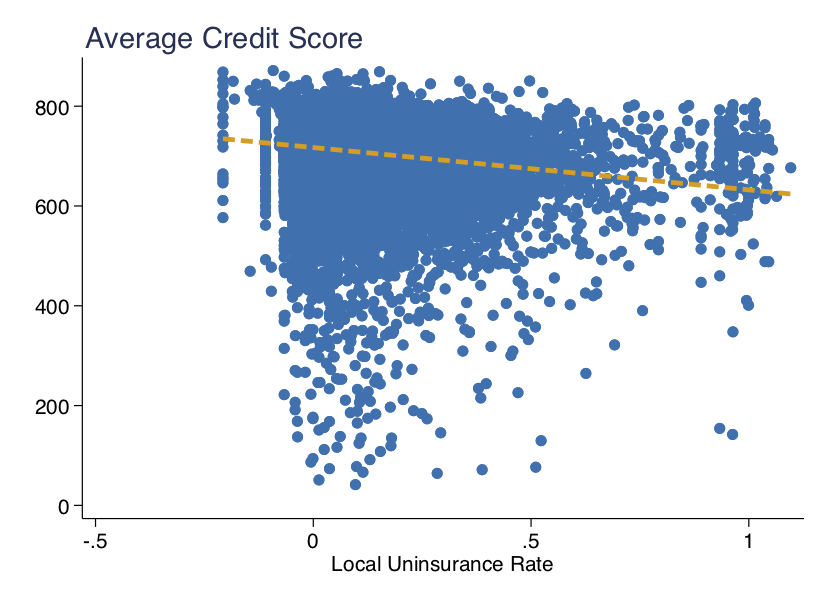
\includegraphics[width=\linewidth]{images/example_scatter4.png}
      }
  \end{column}
\end{columns}
\end{frame}


\begin{frame}{Can we do more?}
  \begin{wideitemize}
  \item  Residual regression is powerful
  \item Maybe we could use it to do something more flexible?  When I
    plot my data, it's not totally obvious that a straight line is the
    best fit. But it's hard to see because there's so much data.
  \item   Recall that we're acutally interested in conditional expectation functions -- e.g. $E(Y | D )$
    \begin{itemize}
    \item   What's a way to  approximate this?
    \end{itemize}
  \end{wideitemize}
\end{frame}

\begin{frame}{An aside on non-parametric vs. semiparametric vs. parametric}
  \begin{wideitemize}
  \item What I view as the formal definition:
    \begin{itemize}
    \item Parametric: model where data generating process is specified as finite dimensional. Hence,
      $$ Y_{i} = D_{i}\beta + \epsilon_{i}, \qquad \epsilon_{i} \sim \mathcal{N}(0, \sigma^{2})$$
      is a fully parametric model (conditional on $D$)
    \item Non-parametric: model where the data generating process is specified as infinite dimensional. E.g.
      $$ Y_{i} = F(D_{i},\theta_{i})$$
      where $\theta_{i}$ is infinite-dimensional parameter
    \item Semi-parametric: a combination. E.g. even OLS with robust standard errors:
      $$ Y_{i} = D_{i}\beta + \epsilon_{i}, \qquad \epsilon_{i} \sim F(\theta_{i}),$$
      where $\theta_{i}$ is infinite dimensional and $\beta$ is finite dimensional
    \end{itemize}
  \item Important to distinguish between \emph{nuisance} parameters
    (e.g. we don't care about actually estimating $\theta_{i}$ in the
    robust standard error example) and parameters of interest. 
  \end{wideitemize}
\end{frame}

\begin{frame}{Binscatter approach}
  \begin{columns}[T] % align columns
    \begin{column}{.5\textwidth}
      $$ Y_{i} = f(D_{i},\theta) + \epsilon_{i}$$
      \vspace{-10pt}
  \begin{wideitemize}
  \item There are a number of ways to approximate this function in the econometrics literature
    \begin{itemize}
    \item One common approach is called \emph{binscatter}, which uses
      spaced bins to construct means
    \end{itemize}
  \item Why is this useful? Well, much of the time in our plots it is
    hard to see the underlying conditional expectation function.
  \item The dots reflects averages within 20 equally spaced quantiles
    \begin{itemize}
    \item Idea: points reflect $f(D_{i})$
    \end{itemize}
  \end{wideitemize}
  \end{column}%
  \hfill%
  \begin{column}{.5\textwidth}
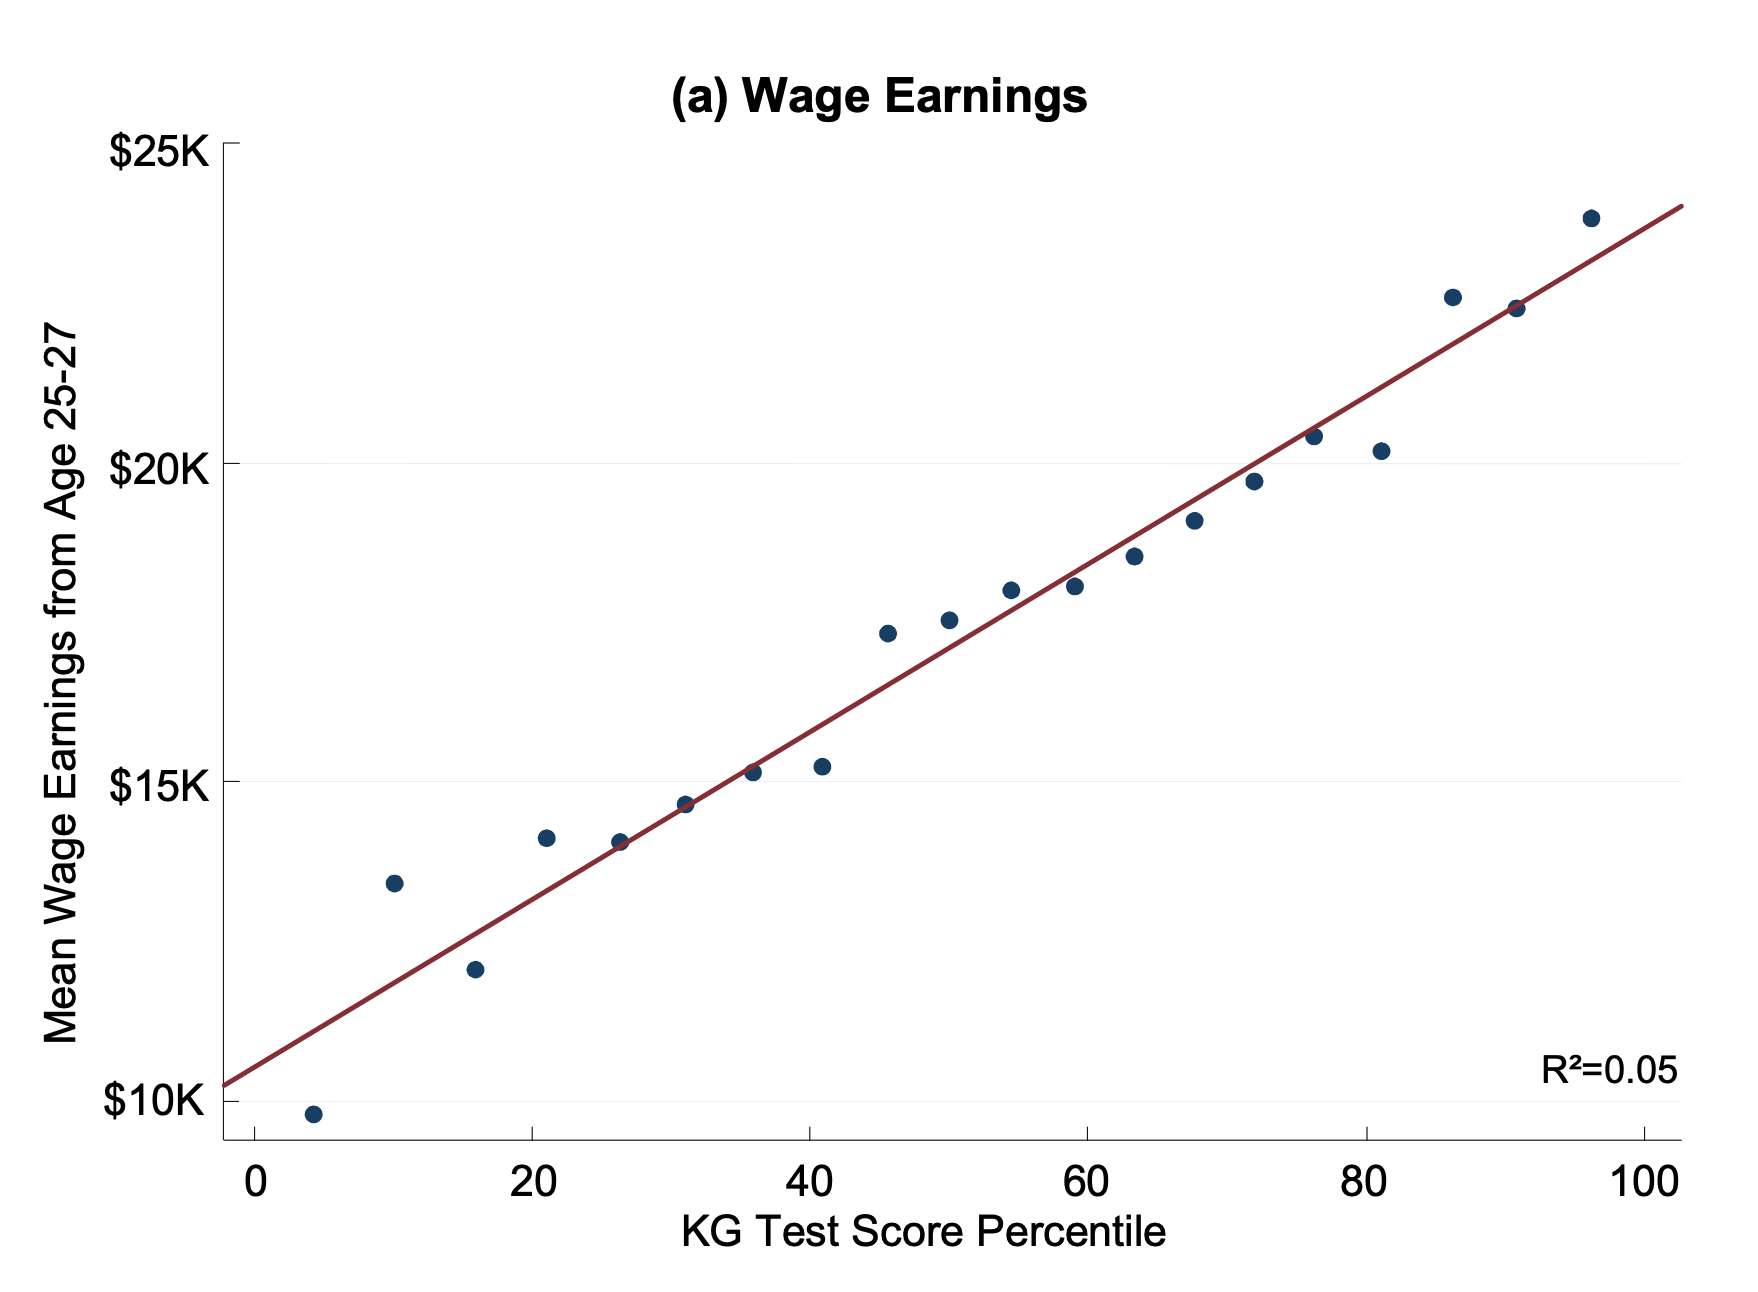
\includegraphics[width=\linewidth]{images/first_binscatter.png}
Chetty et al. (2011) - Kindergarten scores on adult earnings
  \end{column}
\end{columns}
\end{frame}

\begin{frame}{Binscatter approach}
  \begin{columns}[T] % align columns
    \begin{column}{.5\textwidth}
      \begin{wideitemize}
      \item Two things worth noting from this (very nice) graph
        \begin{itemize}
        \item The $R^2$ is not enormous, which suggests lots of unexplained variation
        \item We don't have a good reason for the bin choice
        \end{itemize}
      \item In a discrete case, the bin choice is obvious
        \begin{itemize}
        \item Non-parametrics is (easier) when discrete!
        \end{itemize}
      \item So what's going on under the hood?
  \end{wideitemize}
  \end{column}%
  \hfill%
  \begin{column}{.5\textwidth}
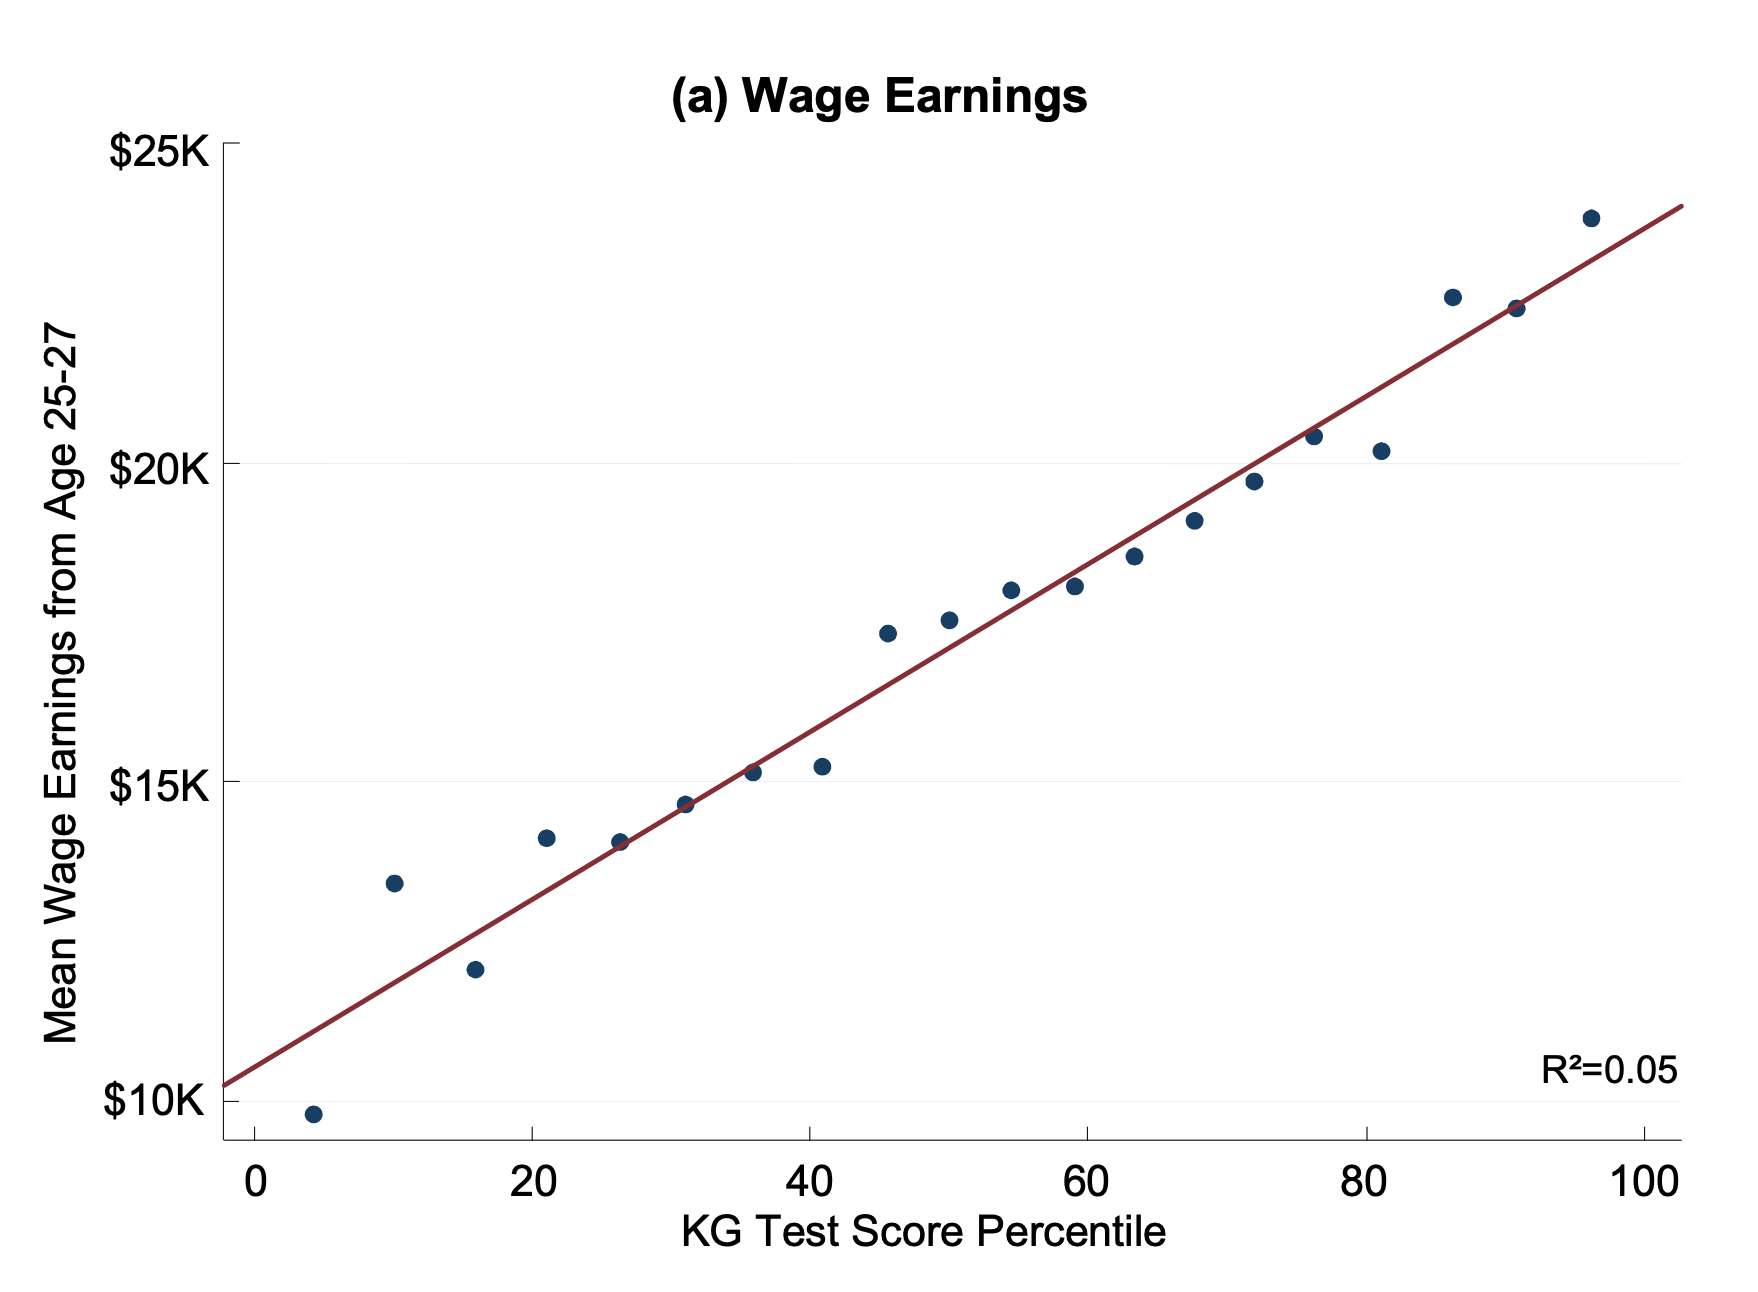
\includegraphics[width=\linewidth]{images/first_binscatter.png}
Chetty et al. (2011) - Kindergarten scores on adult earnings
  \end{column}
\end{columns}
\end{frame}

\begin{frame}{How a binscatter graph is made (Cattaneo et al. (2019)}
  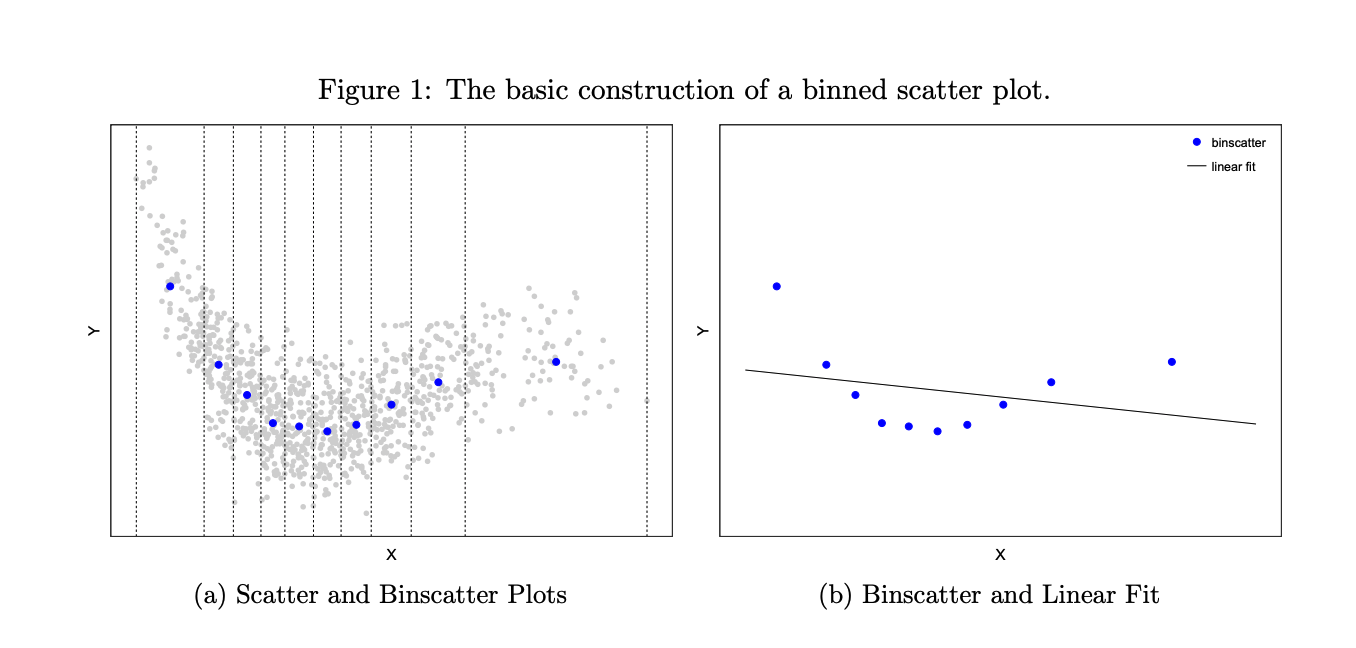
\includegraphics[width=\linewidth]{images/binscatter_crump.png}
\end{frame}


\begin{frame}{Start with binscatter}
  \begin{columns}[T] % align columns
    \begin{column}{.5\textwidth}
      \begin{wideitemize}
      \item<1-> Choice of bin is not obvious
      \item<1-> How you pick bins can influence interpretation
      \item<3-> This is a statistical problem! 
  \end{wideitemize}
  \end{column}%
  \hfill%
  \begin{column}{.5\textwidth}
    \only<1>{
      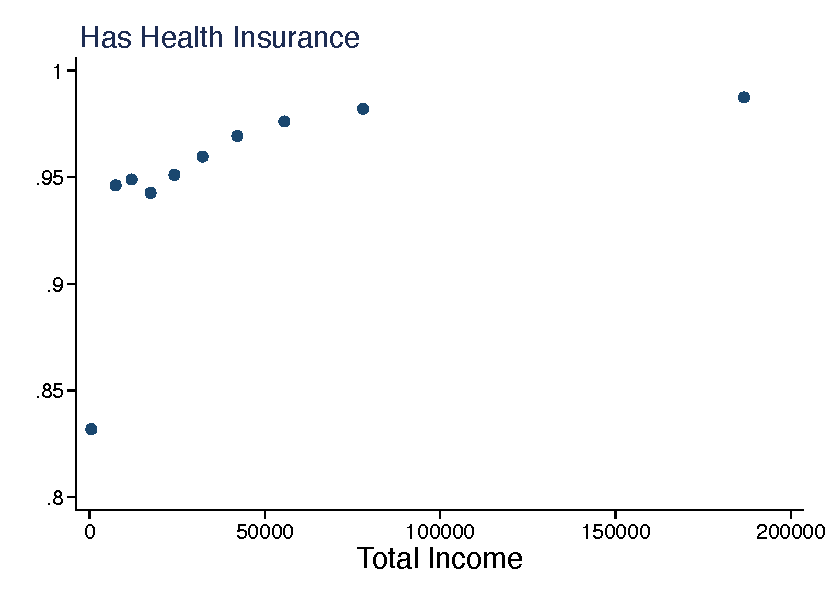
\includegraphics[width=\linewidth]{images/binscatter_insurance1.pdf}
      income on health insurance, 10 bins      
      }
    \only<2>{
      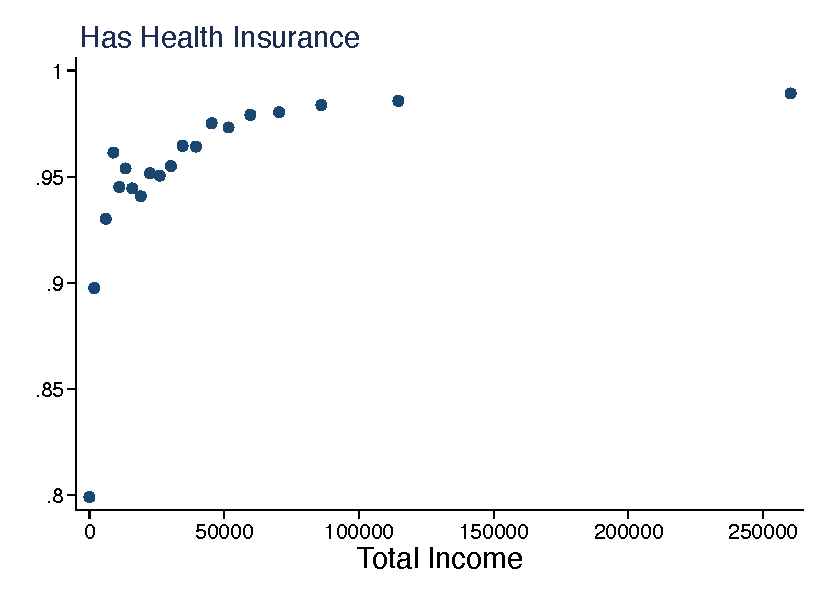
\includegraphics[width=\linewidth]{images/binscatter_insurance2.pdf}
    income on health insurance, 20 bins            
      }
    \only<3>{
      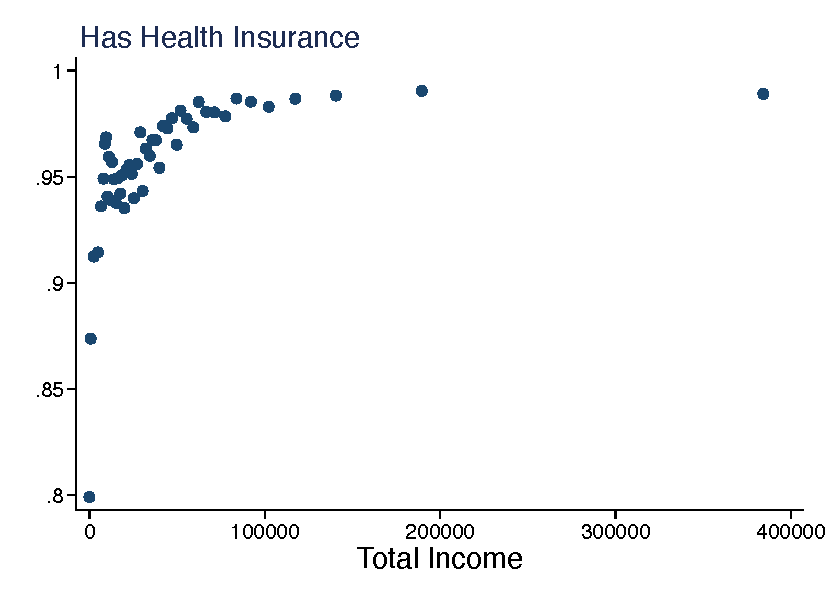
\includegraphics[width=\linewidth]{images/binscatter_insurance3.pdf}
    income on health insurance, 50 bins            
      }
  \end{column}
\end{columns}
\end{frame}

\begin{frame}{Cattaneo et al. ``On Binscatter''}
  \begin{columns}[T] % align columns
    \begin{column}{.5\textwidth}
      \begin{wideitemize}
      \item Paper provides several generalizations to binscatter approach
      \item First contribution: highlight that the ``traditional''
        binscatter approach is presenting a particular non-parametric
        estimation
      \item Initially assumes that constant within bin
        \begin{itemize}
        \item Not crazy! But could do more. 
        \end{itemize}
      \item Piece-wise functions can be made very flexible
  \end{wideitemize}
  \end{column}%
  \hfill%
  \begin{column}{.5\textwidth}
    \only<1>{
      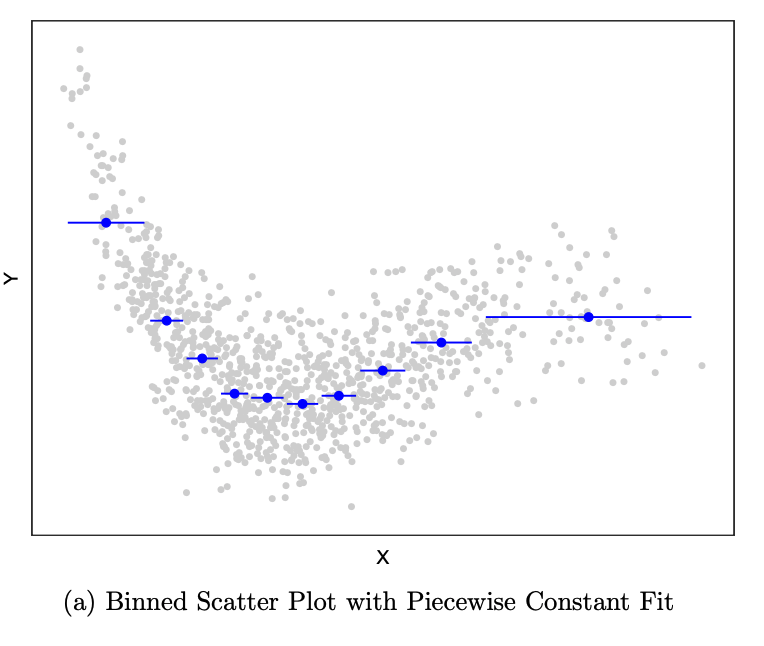
\includegraphics[width=\linewidth]{images/binscatter_crump_bins1.png}
      }
    \only<2>{
      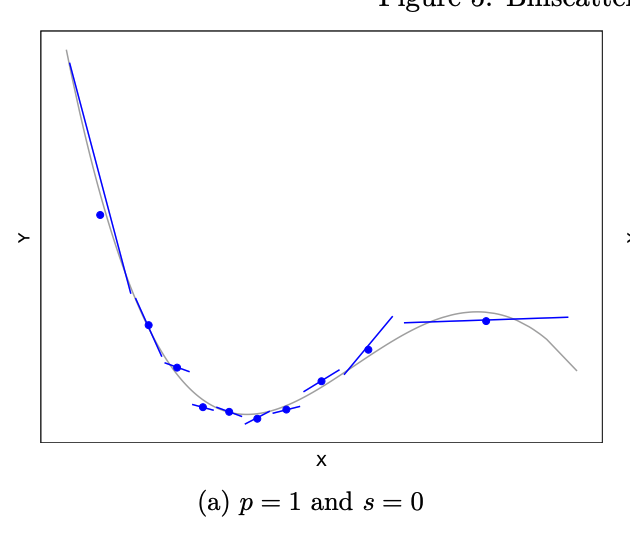
\includegraphics[width=\linewidth]{images/binscatter_crump_bins2.png}
      }
    \only<3>{
      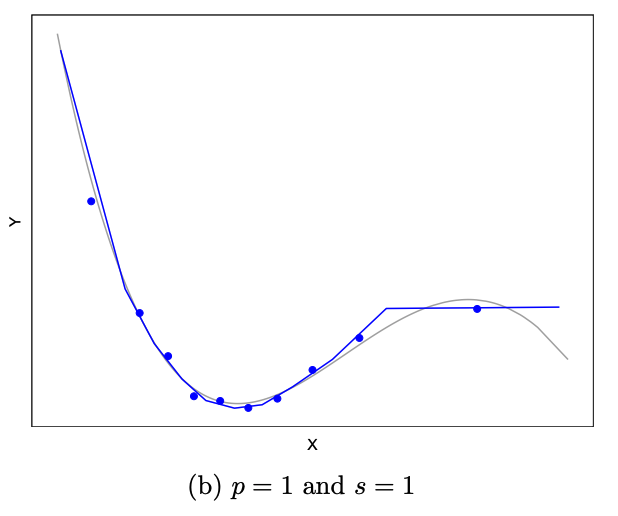
\includegraphics[width=\linewidth]{images/binscatter_crump_bins3.png}
      }
  \end{column}
\end{columns}
  
\end{frame}

\begin{frame}{Cattaneo et al. ``On Binscatter''}
  \begin{columns}[T] % align columns
    \begin{column}{.7\textwidth}
      \begin{wideitemize}
      \item Second contribution: Choosing bins!
      \item Reframe as non-parametric problem. Estimation problem is tradeoff:
        \begin{itemize}
        \item  bias (picking too few bins makes your function off)
        \item and noise (pick too many bins and they're very noisy)
        \end{itemize}
      \item In canonical binscatter, $\approx n^{1/3}$
        \begin{itemize}
        \item This is data driven tuning, so you tie your hands a bit and
          avoid data-snooping issues!
        \end{itemize}
  \end{wideitemize}
  \end{column}%
  \hfill%
  \begin{column}{.5\textwidth}
  \end{column}
\end{columns}
\end{frame}

\begin{frame}{Cattaneo et al. ``On Binscatter''}
  \begin{columns}[T] % align columns
    \begin{column}{.5\textwidth}
      \begin{wideitemize}
      \item Third contribution: back to residual regression
      \item Recall our approach was to residualize $D_{i}$ by our
        controls to do residual regression
        \begin{itemize}
        \item Exploiting Frisch-Waugh-Lovell theorem
        \end{itemize}
        $$ Y_{i} = f(D_{i},\theta) + W_{i}\beta + \epsilon_{i}$$
      \item In this setting, you can't residual $D_{i}$ and get back
        the function $f$ if $f$ is non-linear
        \begin{itemize}
        \item Unfortunately, this is what historically has been the default in Stata package
        \end{itemize}
      \item Correct way to view this -- imagine binning $D_{i}$ and
        running the regression. You want to plot the coefficients
  \end{wideitemize}
  \end{column}%
  \hfill%
  \begin{column}{.5\textwidth}
    \only<2>{
      Comparison of methods:
      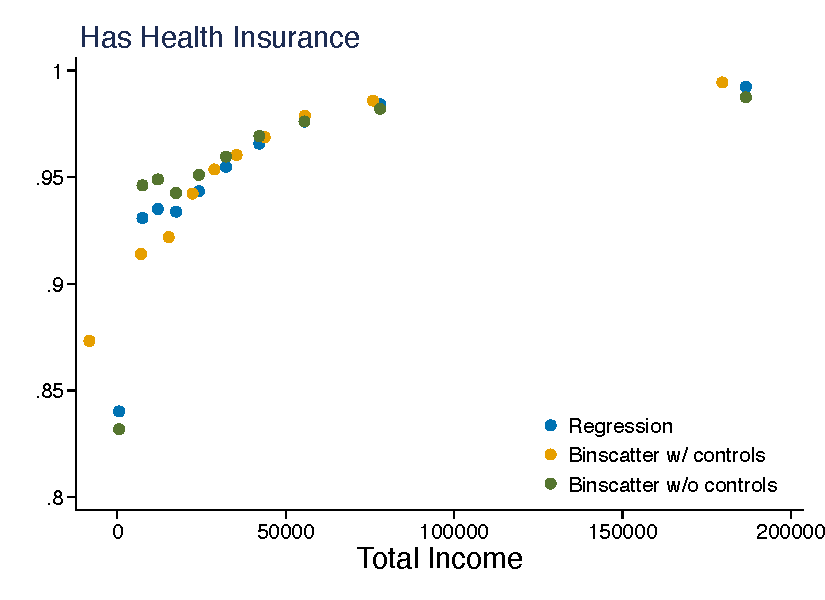
\includegraphics[width=\linewidth]{images/binscatter_insurance_controls_comparison.pdf}
      Controls: age, sex, and state of residence
      }
  \end{column}
\end{columns}
\end{frame}



\begin{frame}{Cattaneo et al. ``On Binscatter''}
  \begin{columns}[T] % align columns
    \begin{column}{.5\textwidth}
      \begin{wideitemize}
      \item Final contribiution: testing the CEF
      \item By defining the estimand, we can actually test properties
        of it
        \begin{itemize}
        \item Confidence intervals
        \item Test monotonicity
        \end{itemize}
      \item We actually see a noticeable dip across income -- maybe
        driven by Medicaid eligibility thresholds?
      \item Code for this is all available here: \url{https://nppackages.github.io/binsreg/}
      \item If you just want to fix the FWL issue: \url{https://github.com/mdroste/stata-binscatter2}
  \end{wideitemize}
  \end{column}%
  \hfill%
  \begin{column}{.5\textwidth}
    \only<1>{
      Comparison of methods:
      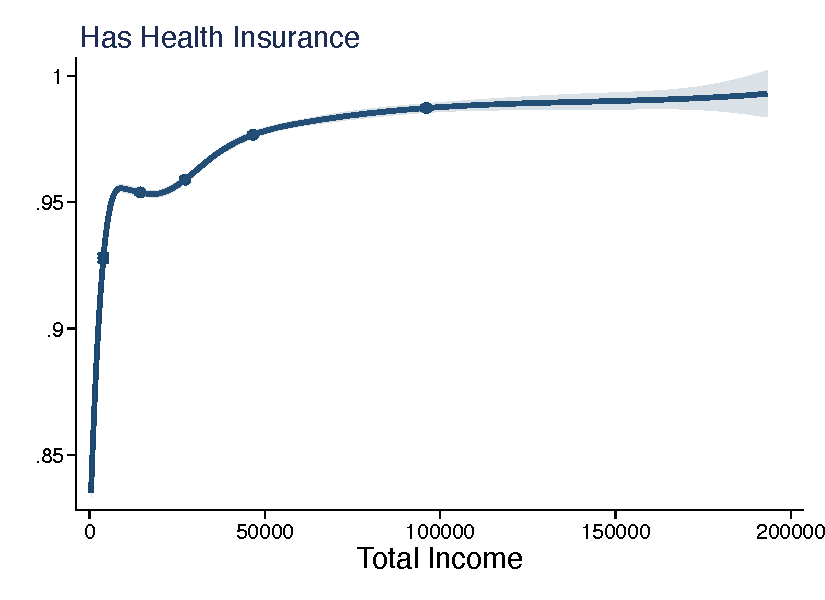
\includegraphics[width=\linewidth]{images/binsreg_insurance_nocontrols.pdf}
      }
    \only<2>{
      Comparison of methods:
      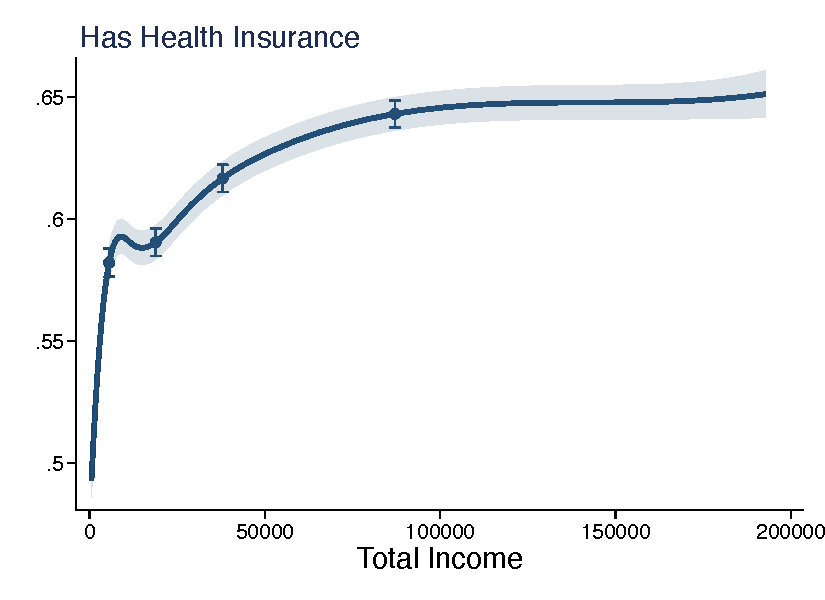
\includegraphics[width=\linewidth]{images/binsreg_insurance_controls.pdf}
      Controls: age, sex, and state of residence
      (Note, level is off b/c program currently does not recenter correctly with covariates)
      }
  \end{column}
\end{columns}
\end{frame}


\begin{frame}{Binscatter}
  \begin{columns}[T] % align columns
    \begin{column}{.5\textwidth}
      \begin{wideitemize}
      \item Key point: Binscatter is super useful, but needs to be done correctly
        \begin{itemize}
        \item Do not mess up the Frisch-Waugh-Lovell point
        \end{itemize}
      \item Taking serious the estimand adds a lot of tools into your toolset!
      \item But, a lot of times these approaches are buttressing a
        simple reported linear number
        \begin{itemize}
        \item Nuance is important, but a paper has many pieces --
          useful to have summary numbers
        \end{itemize}
  \end{wideitemize}
  \end{column}%
  \hfill%
  \begin{column}{.5\textwidth}
      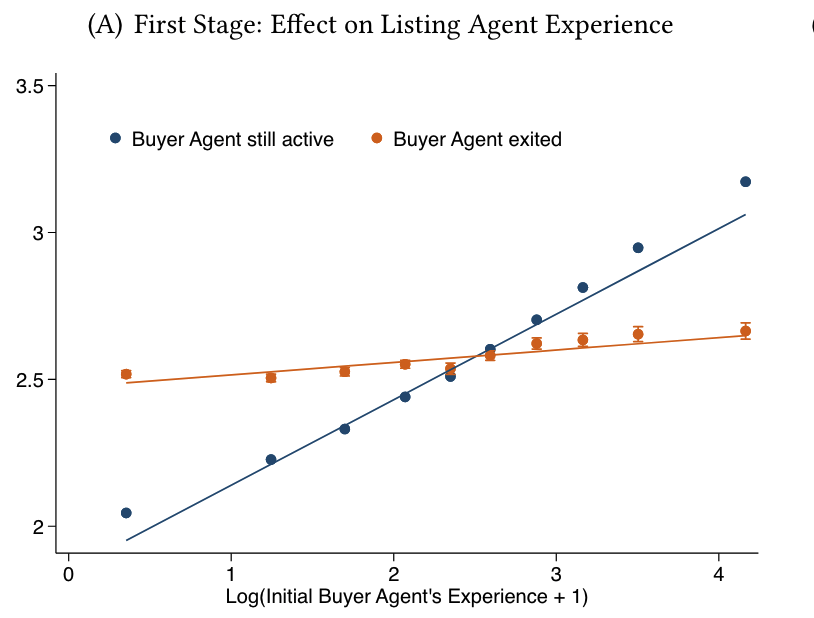
\includegraphics[width=\linewidth]{images/agent_binscatter.png}
  \end{column}
\end{columns}
\end{frame}


\begin{frame}{Why was binscatter so successful?}
  \begin{columns}[T] % align columns
    \begin{column}{.7\textwidth}
      \begin{wideitemize}
      \item As an intellectual history, binscatter approach is a very
        recent innovation in applied work
        \begin{itemize}
        \item Became a staple of much of Raj Chetty and coauthor's work
        \end{itemize}
      \item Extremely successful as an example of improving our data
        visualization to communicate results
        \begin{itemize}
        \item The status quo of big regression tables is \emph{bad}
        \end{itemize}
      \item Will finish by discussing ways to improve visual design
        and improving communication in papers
  \end{wideitemize}
  \end{column}%
  \hfill%
  \begin{column}{.3\textwidth}
          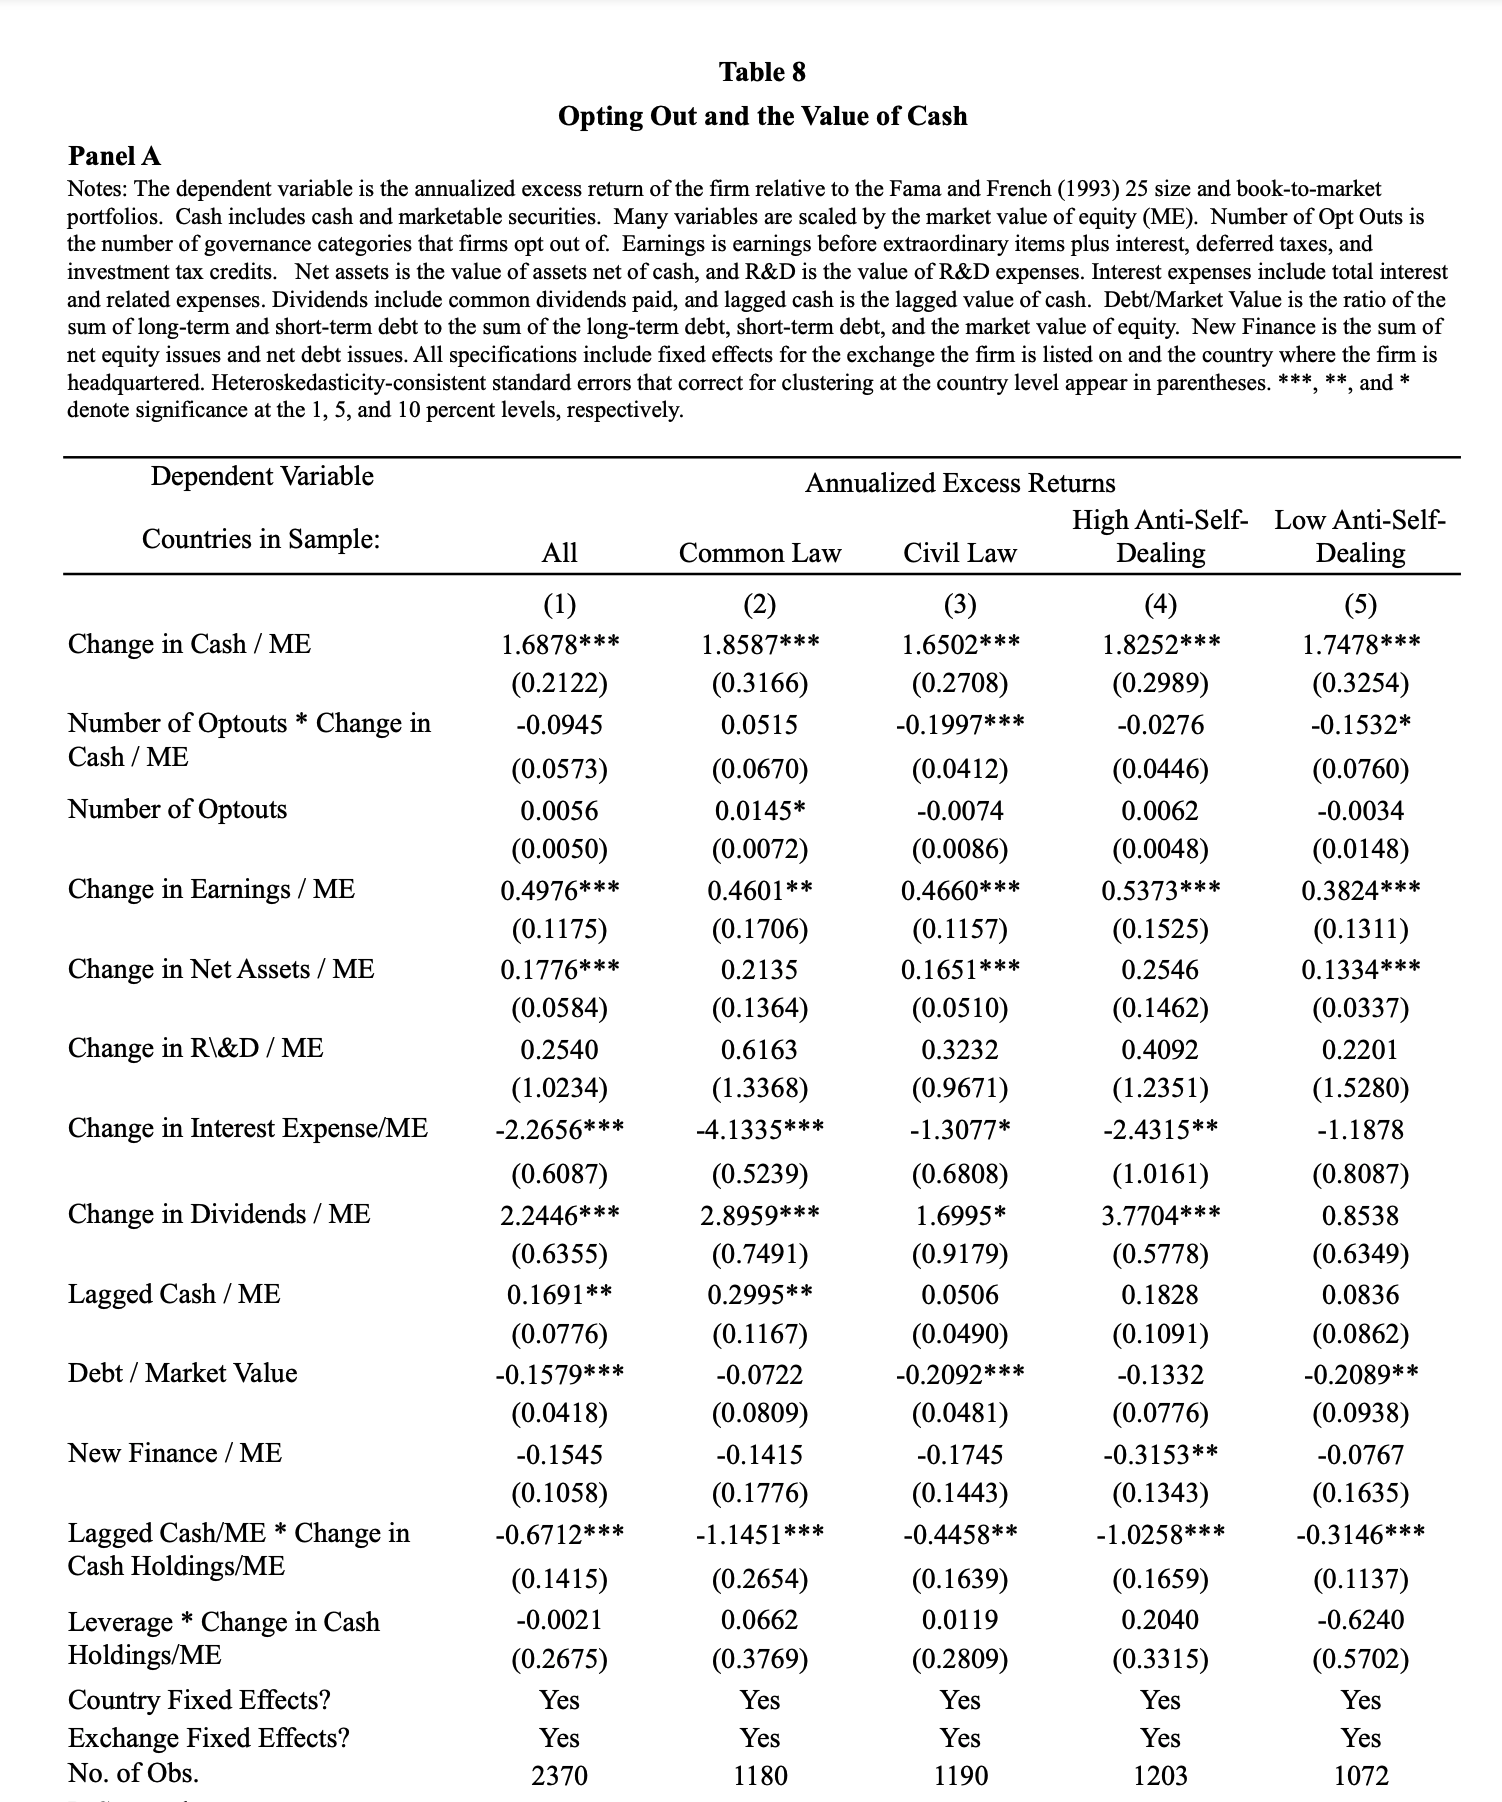
\includegraphics[width=\linewidth]{images/bad_table.png}
  \end{column}
\end{columns}
\end{frame}


\begin{frame}{My design goals}
  \begin{columns}[T] % align columns
    \begin{column}{.6\textwidth}
      \begin{enumerate}
      \item Minimize tables 
      \item Have describable goals for every exhibit
      \item Focus the reader and craft not-ugly figures
        \begin{itemize}
        \item Ideally beautiful, but at minimum not ugly
        \end{itemize}
      \item Do not \emph{mislead} your readers
      \end{enumerate}
      \pause
  \end{column}%
  \hfill%
  \begin{column}{.4\textwidth}
    Within figures, Schwabish's guidelines are excellent:
    \begin{enumerate}
    \item Show the data
    \item Reduce clutter
    \item Integrate graphics and text
    \item Avoid providing extraneous information
    \item Start with grey
    \end{enumerate}
  \end{column}
\end{columns}
\end{frame}

\begin{frame}{1. Minimize Tables}
  \begin{columns}[T] % align columns
    \begin{column}{.6\textwidth}
      \begin{wideitemize}
      \item Tables suck but are important storage units of
        information.
        \begin{itemize}
        \item They should be stored in an online appendix
        \end{itemize}
      \item Tables make it very hard to actually compare results and contrast things
      \item Tables also tend to report things that are unnecessary
        \begin{itemize}
        \item The coefficient on the controls necessary to generate
          strong ignorability are not interpretable in a causal way (Hunermund and Louw (2020))
        \item Why bother reporting them?
        \end{itemize}
      \item Even when not doing regressions!
      \end{wideitemize}
  \end{column}%
  \hfill%
  \begin{column}{.4\textwidth}
  \end{column}
\end{columns}
\end{frame}

\begin{frame}{1. Minimize Tables}
  \begin{columns}[T] % align columns
    \begin{column}{.5\textwidth}
      \begin{wideitemize}
      \item<1-> Several examples of tables vs. regression improvements
      \item<1-> Imbens and Kolesar siulations
      \item<2-> Regression output!
      \item<3-> Can compress a lot of information
      \item<4-> Also can use it for model output  (this is really effective in presentations)
      \end{wideitemize}
  \end{column}%
  \hfill%
  \begin{column}{.5\textwidth}
    \only<1>{
        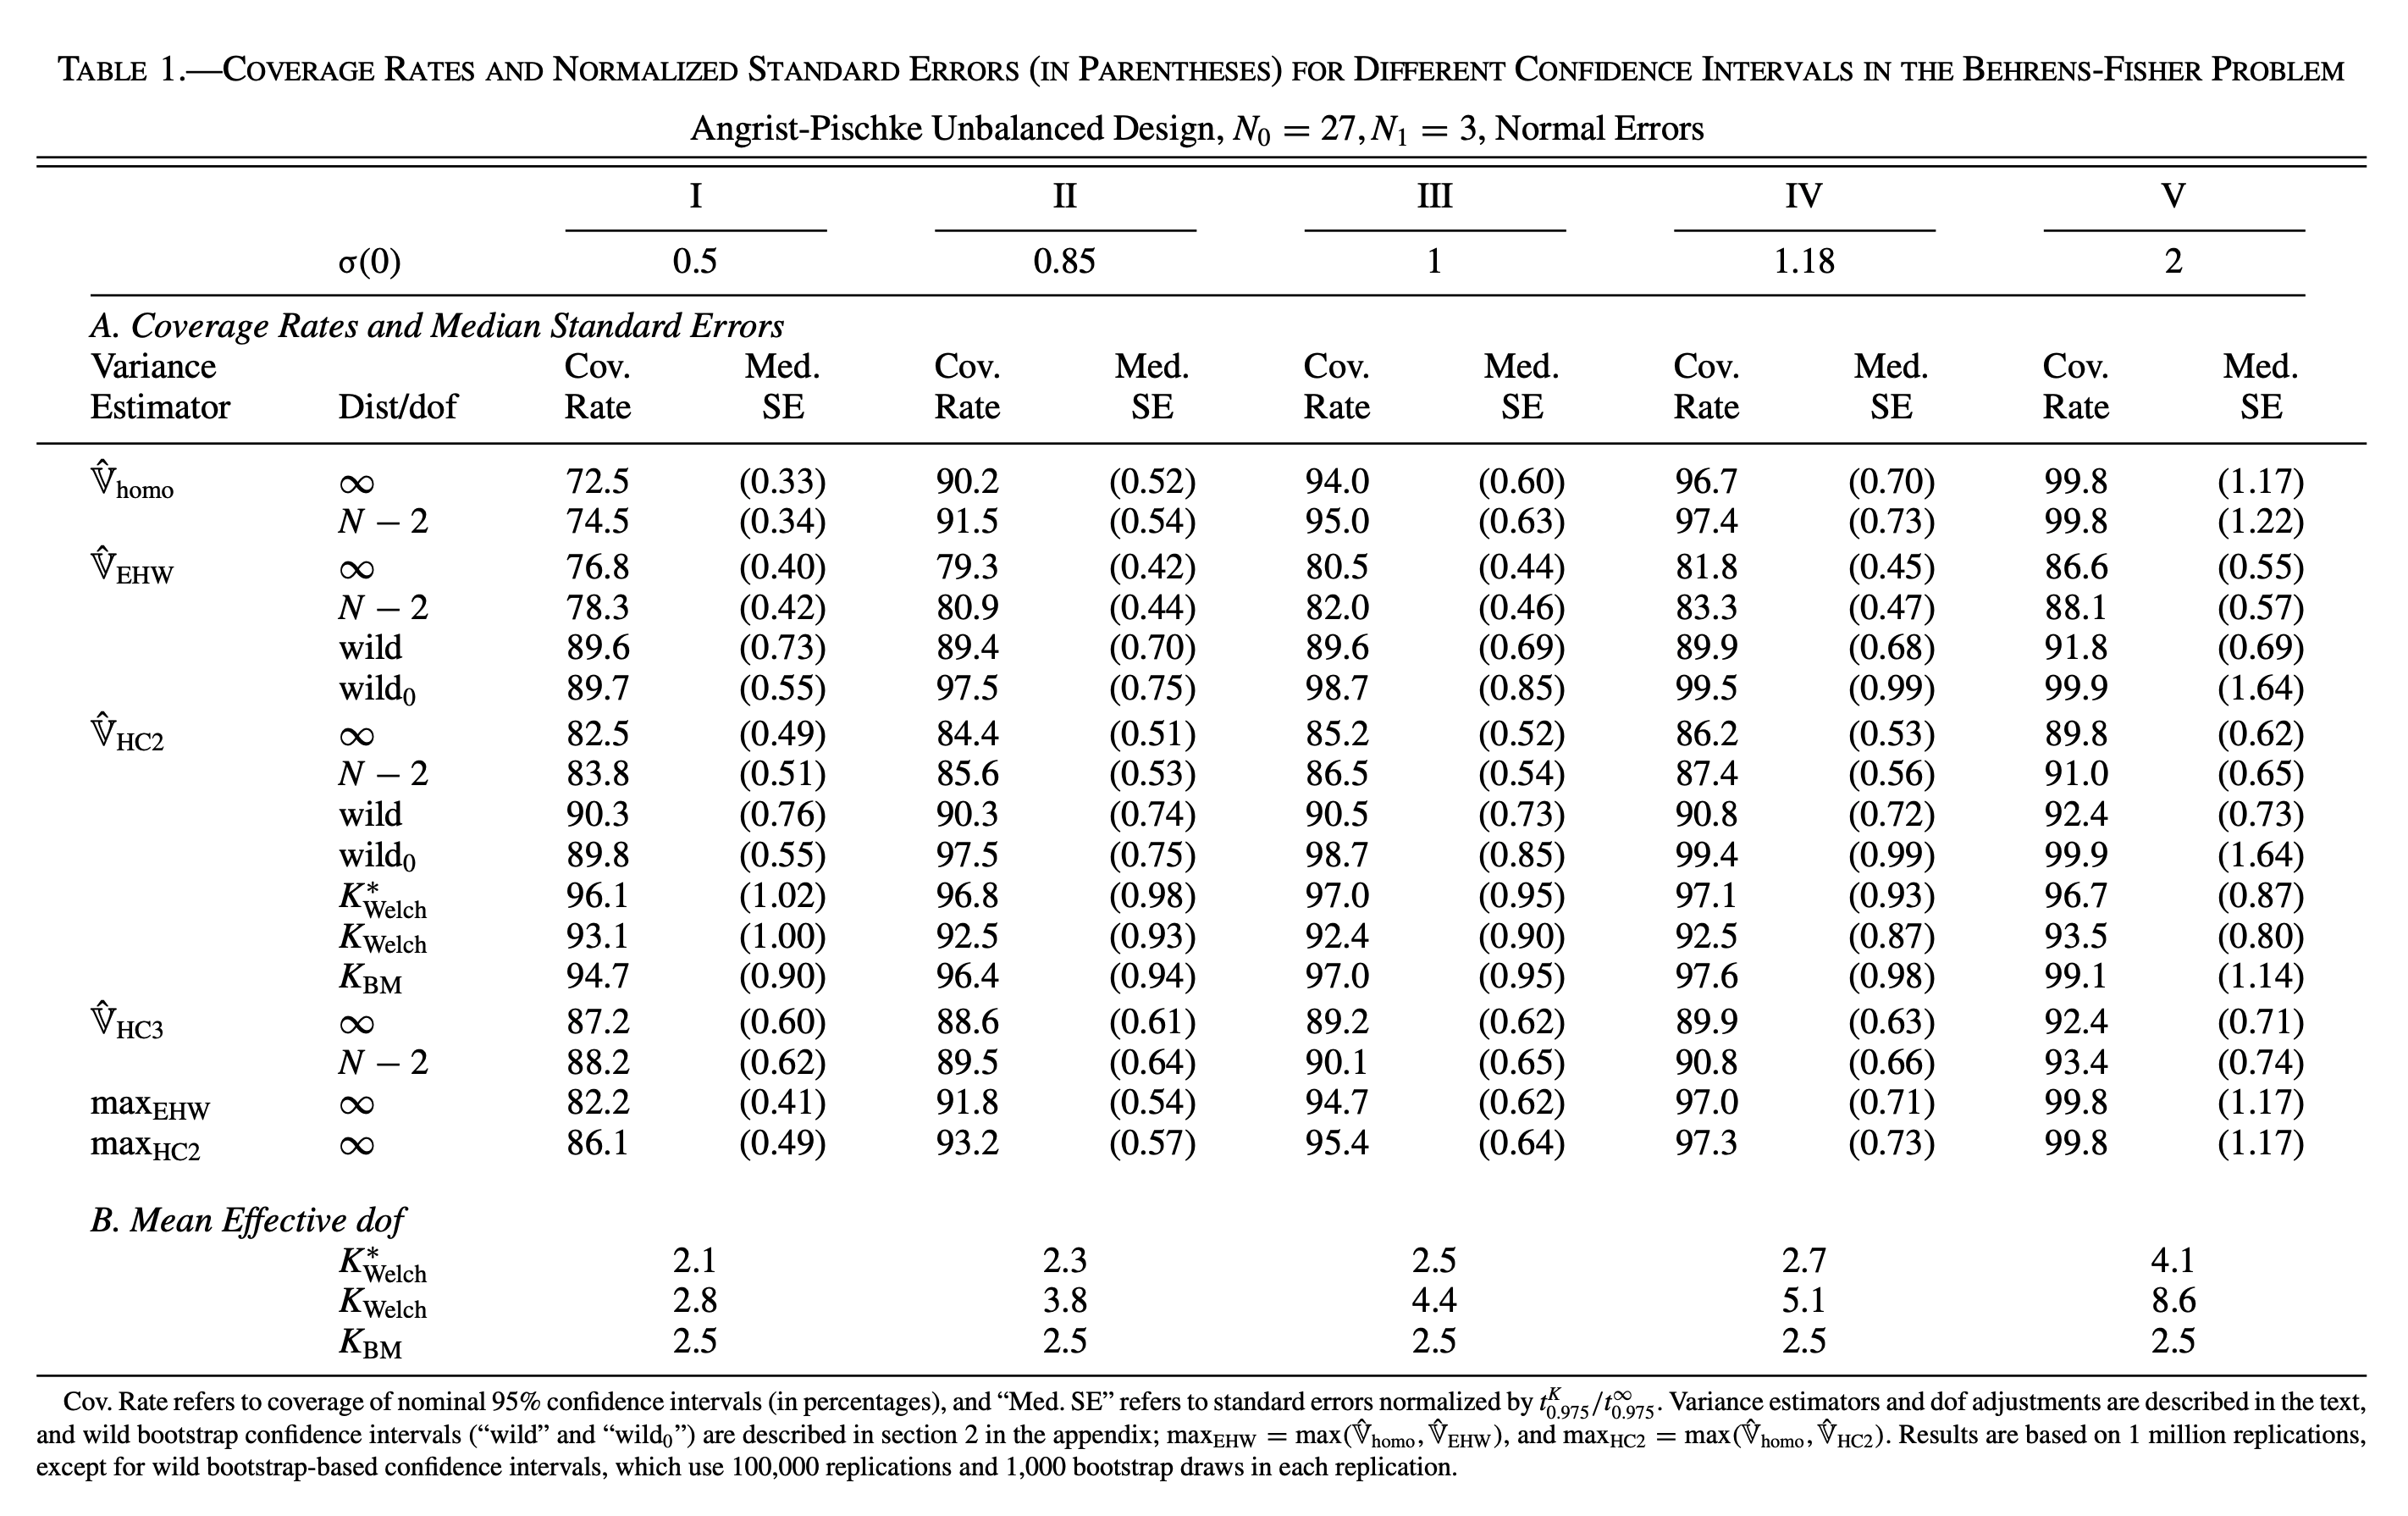
\includegraphics[width=0.8\linewidth]{images/imbenskolsear_coverage_table.png}    \\
        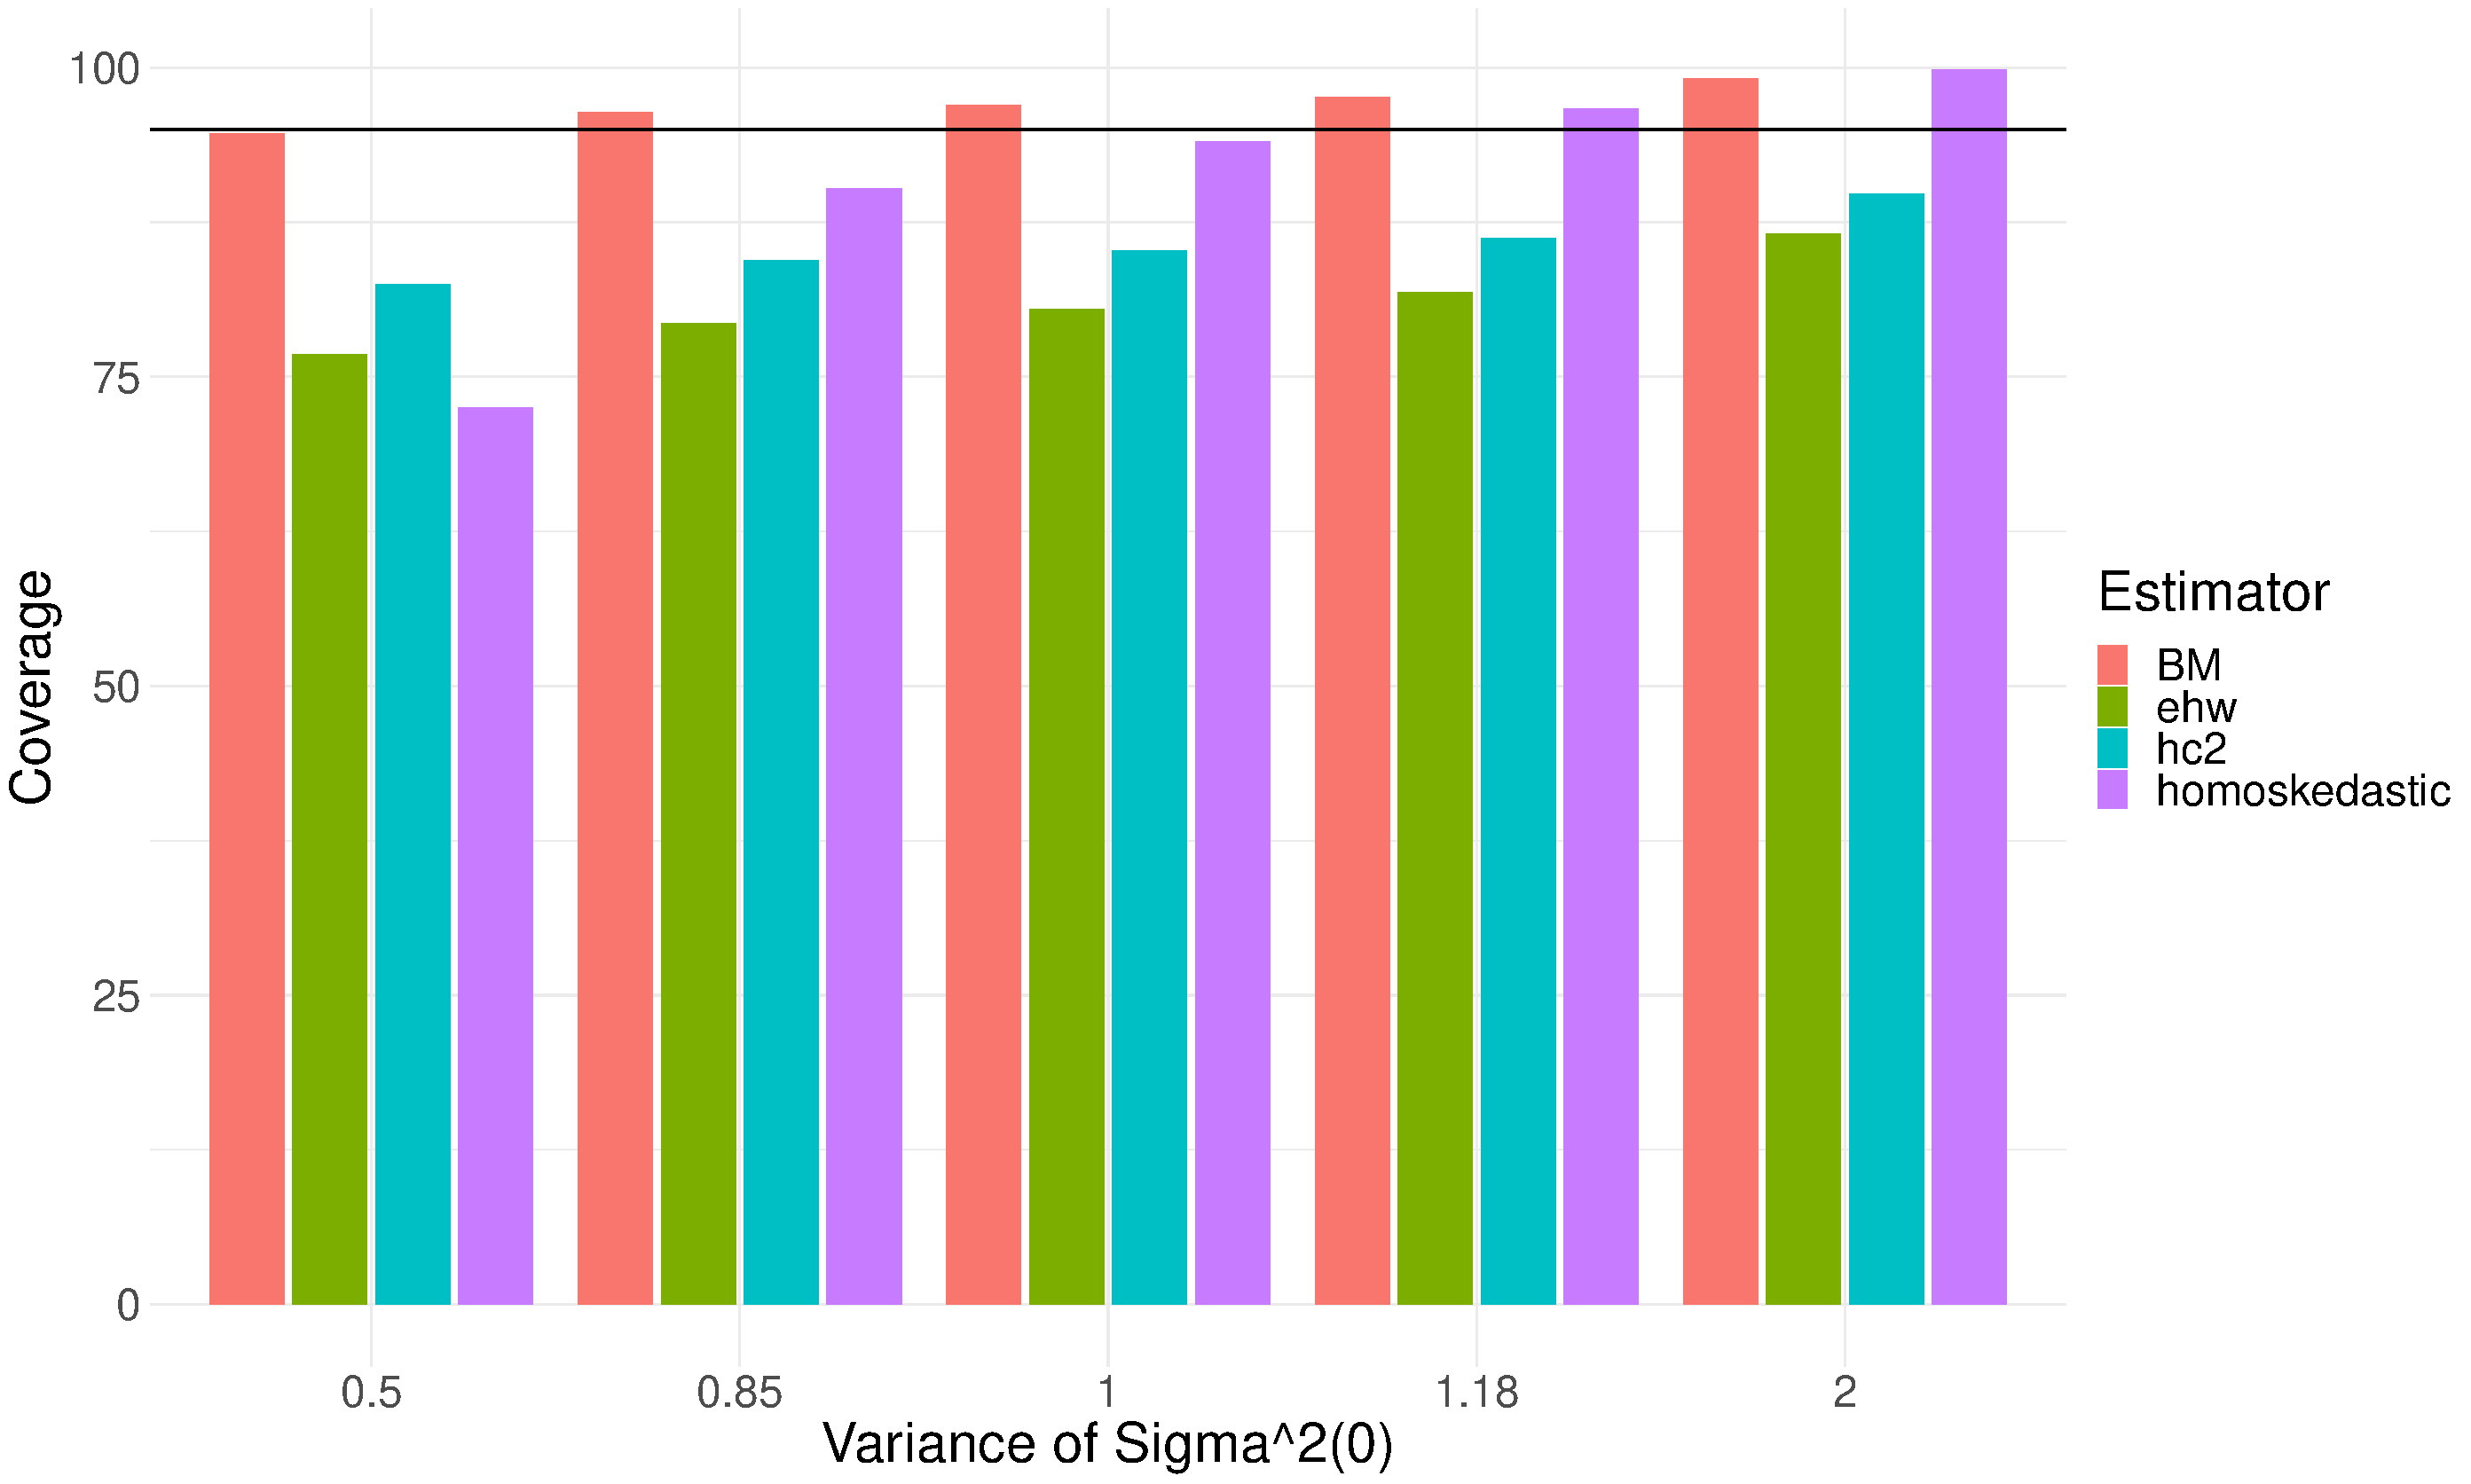
\includegraphics[width=0.9\linewidth]{images/imbenskolesar_coverage.pdf}
      }
    \only<2>{
        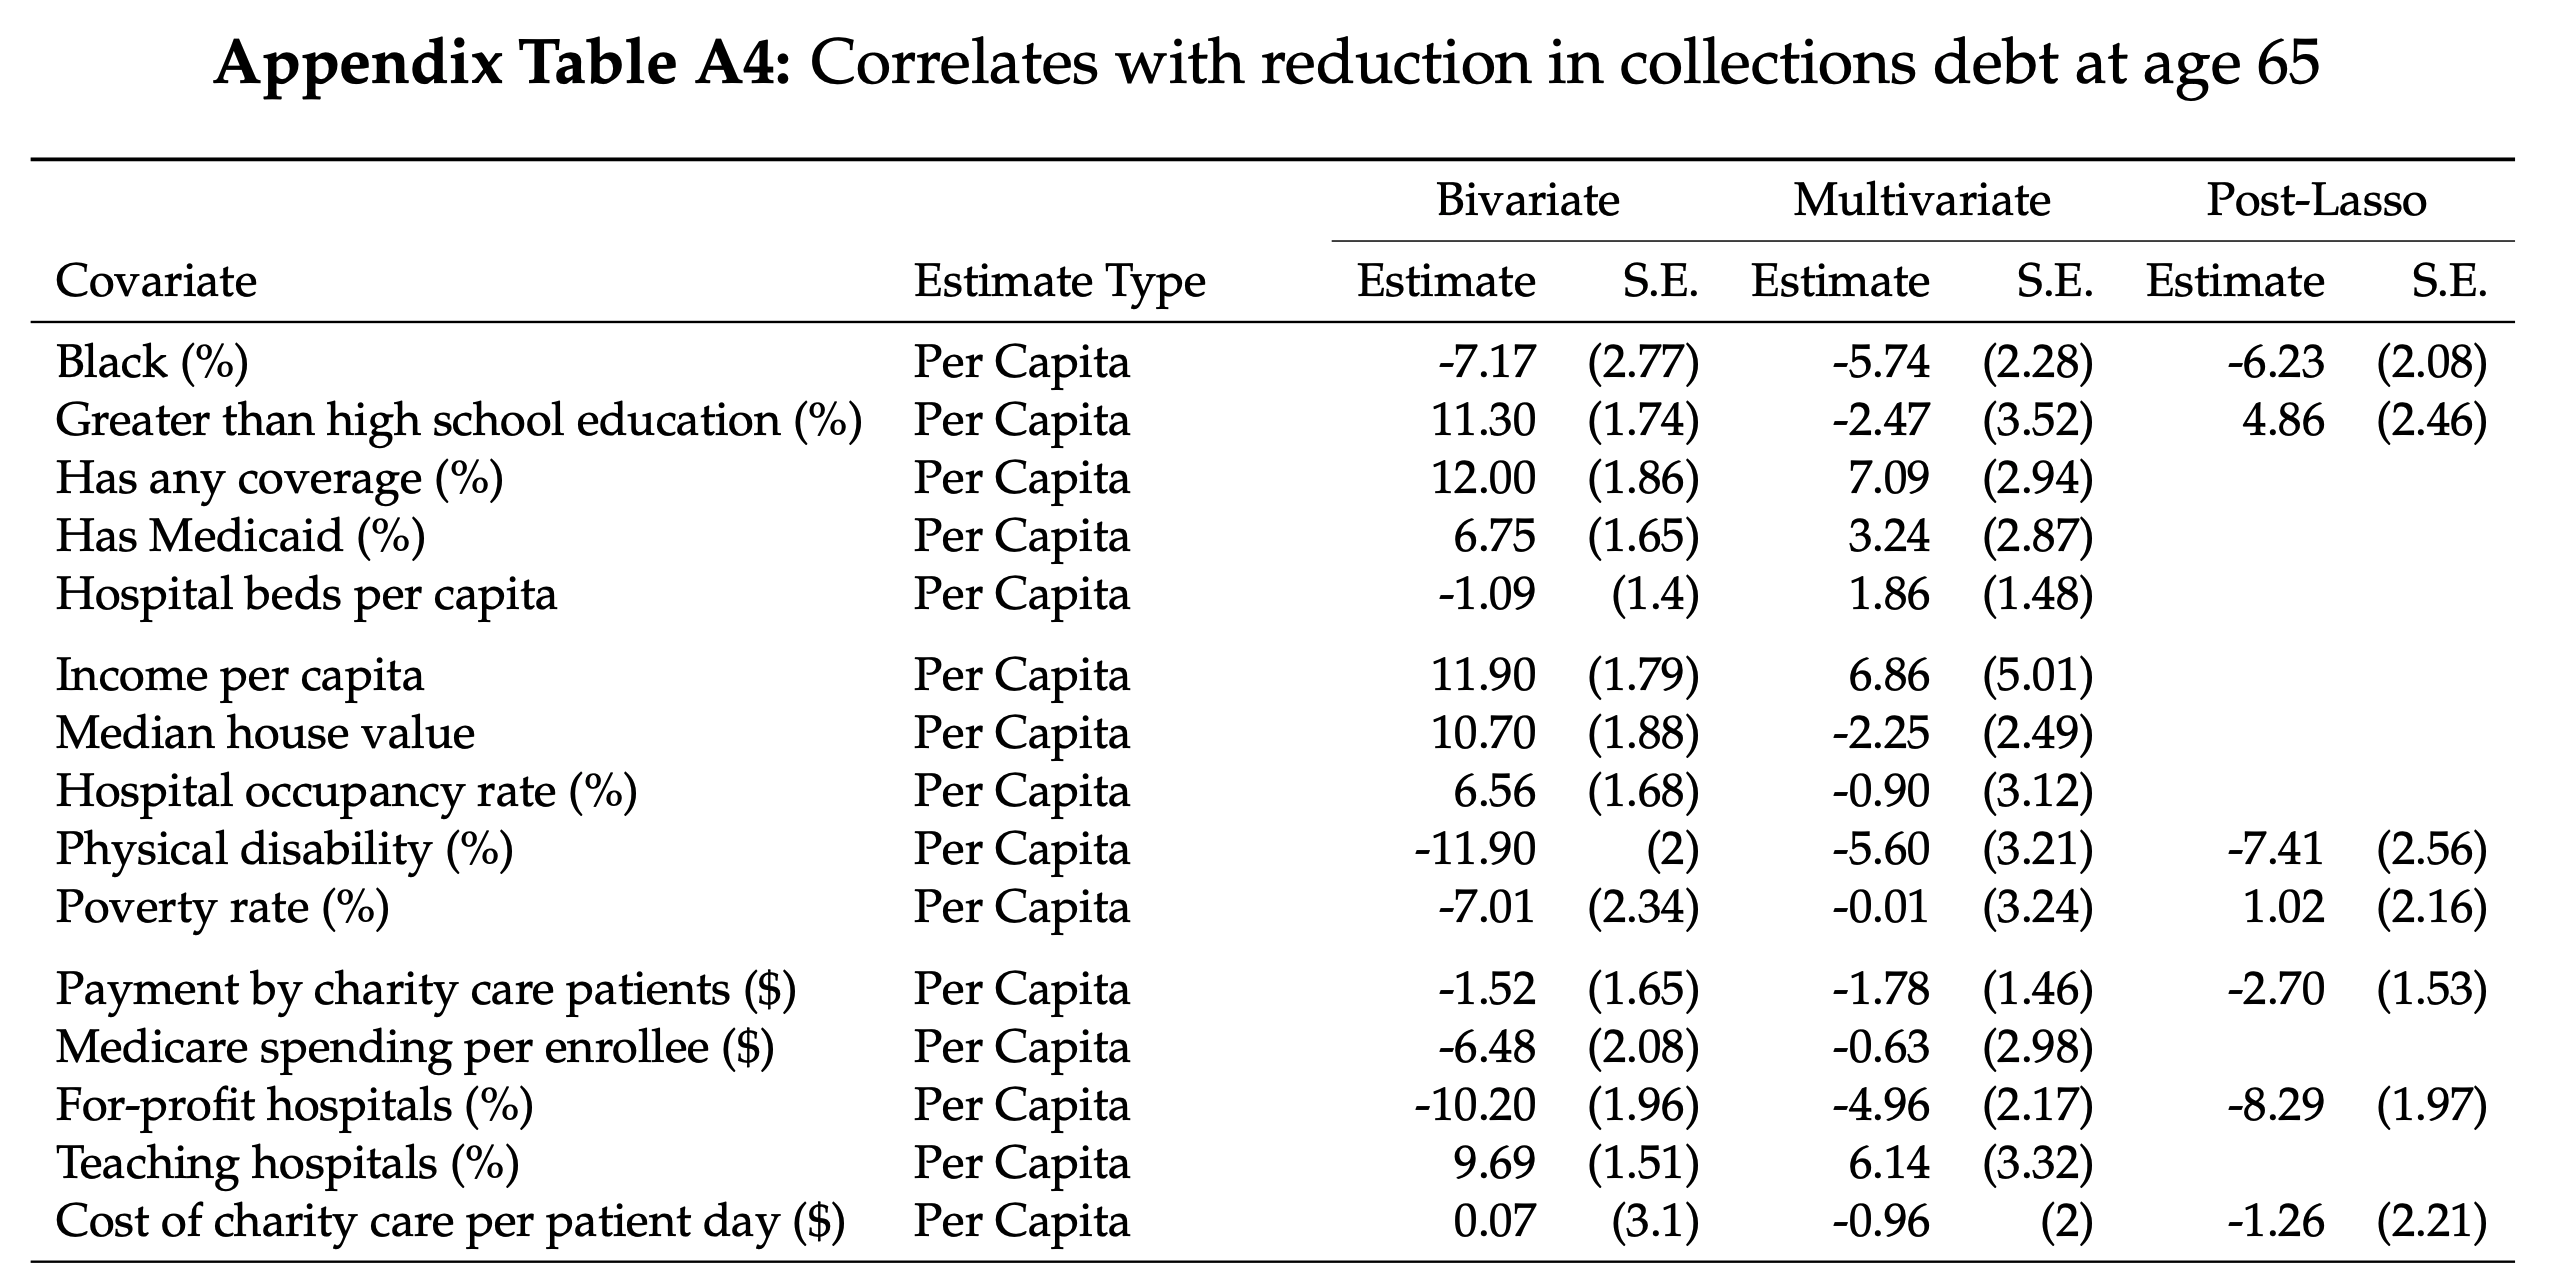
\includegraphics[width=\linewidth]{images/gpw_figure_table.png}    \\
        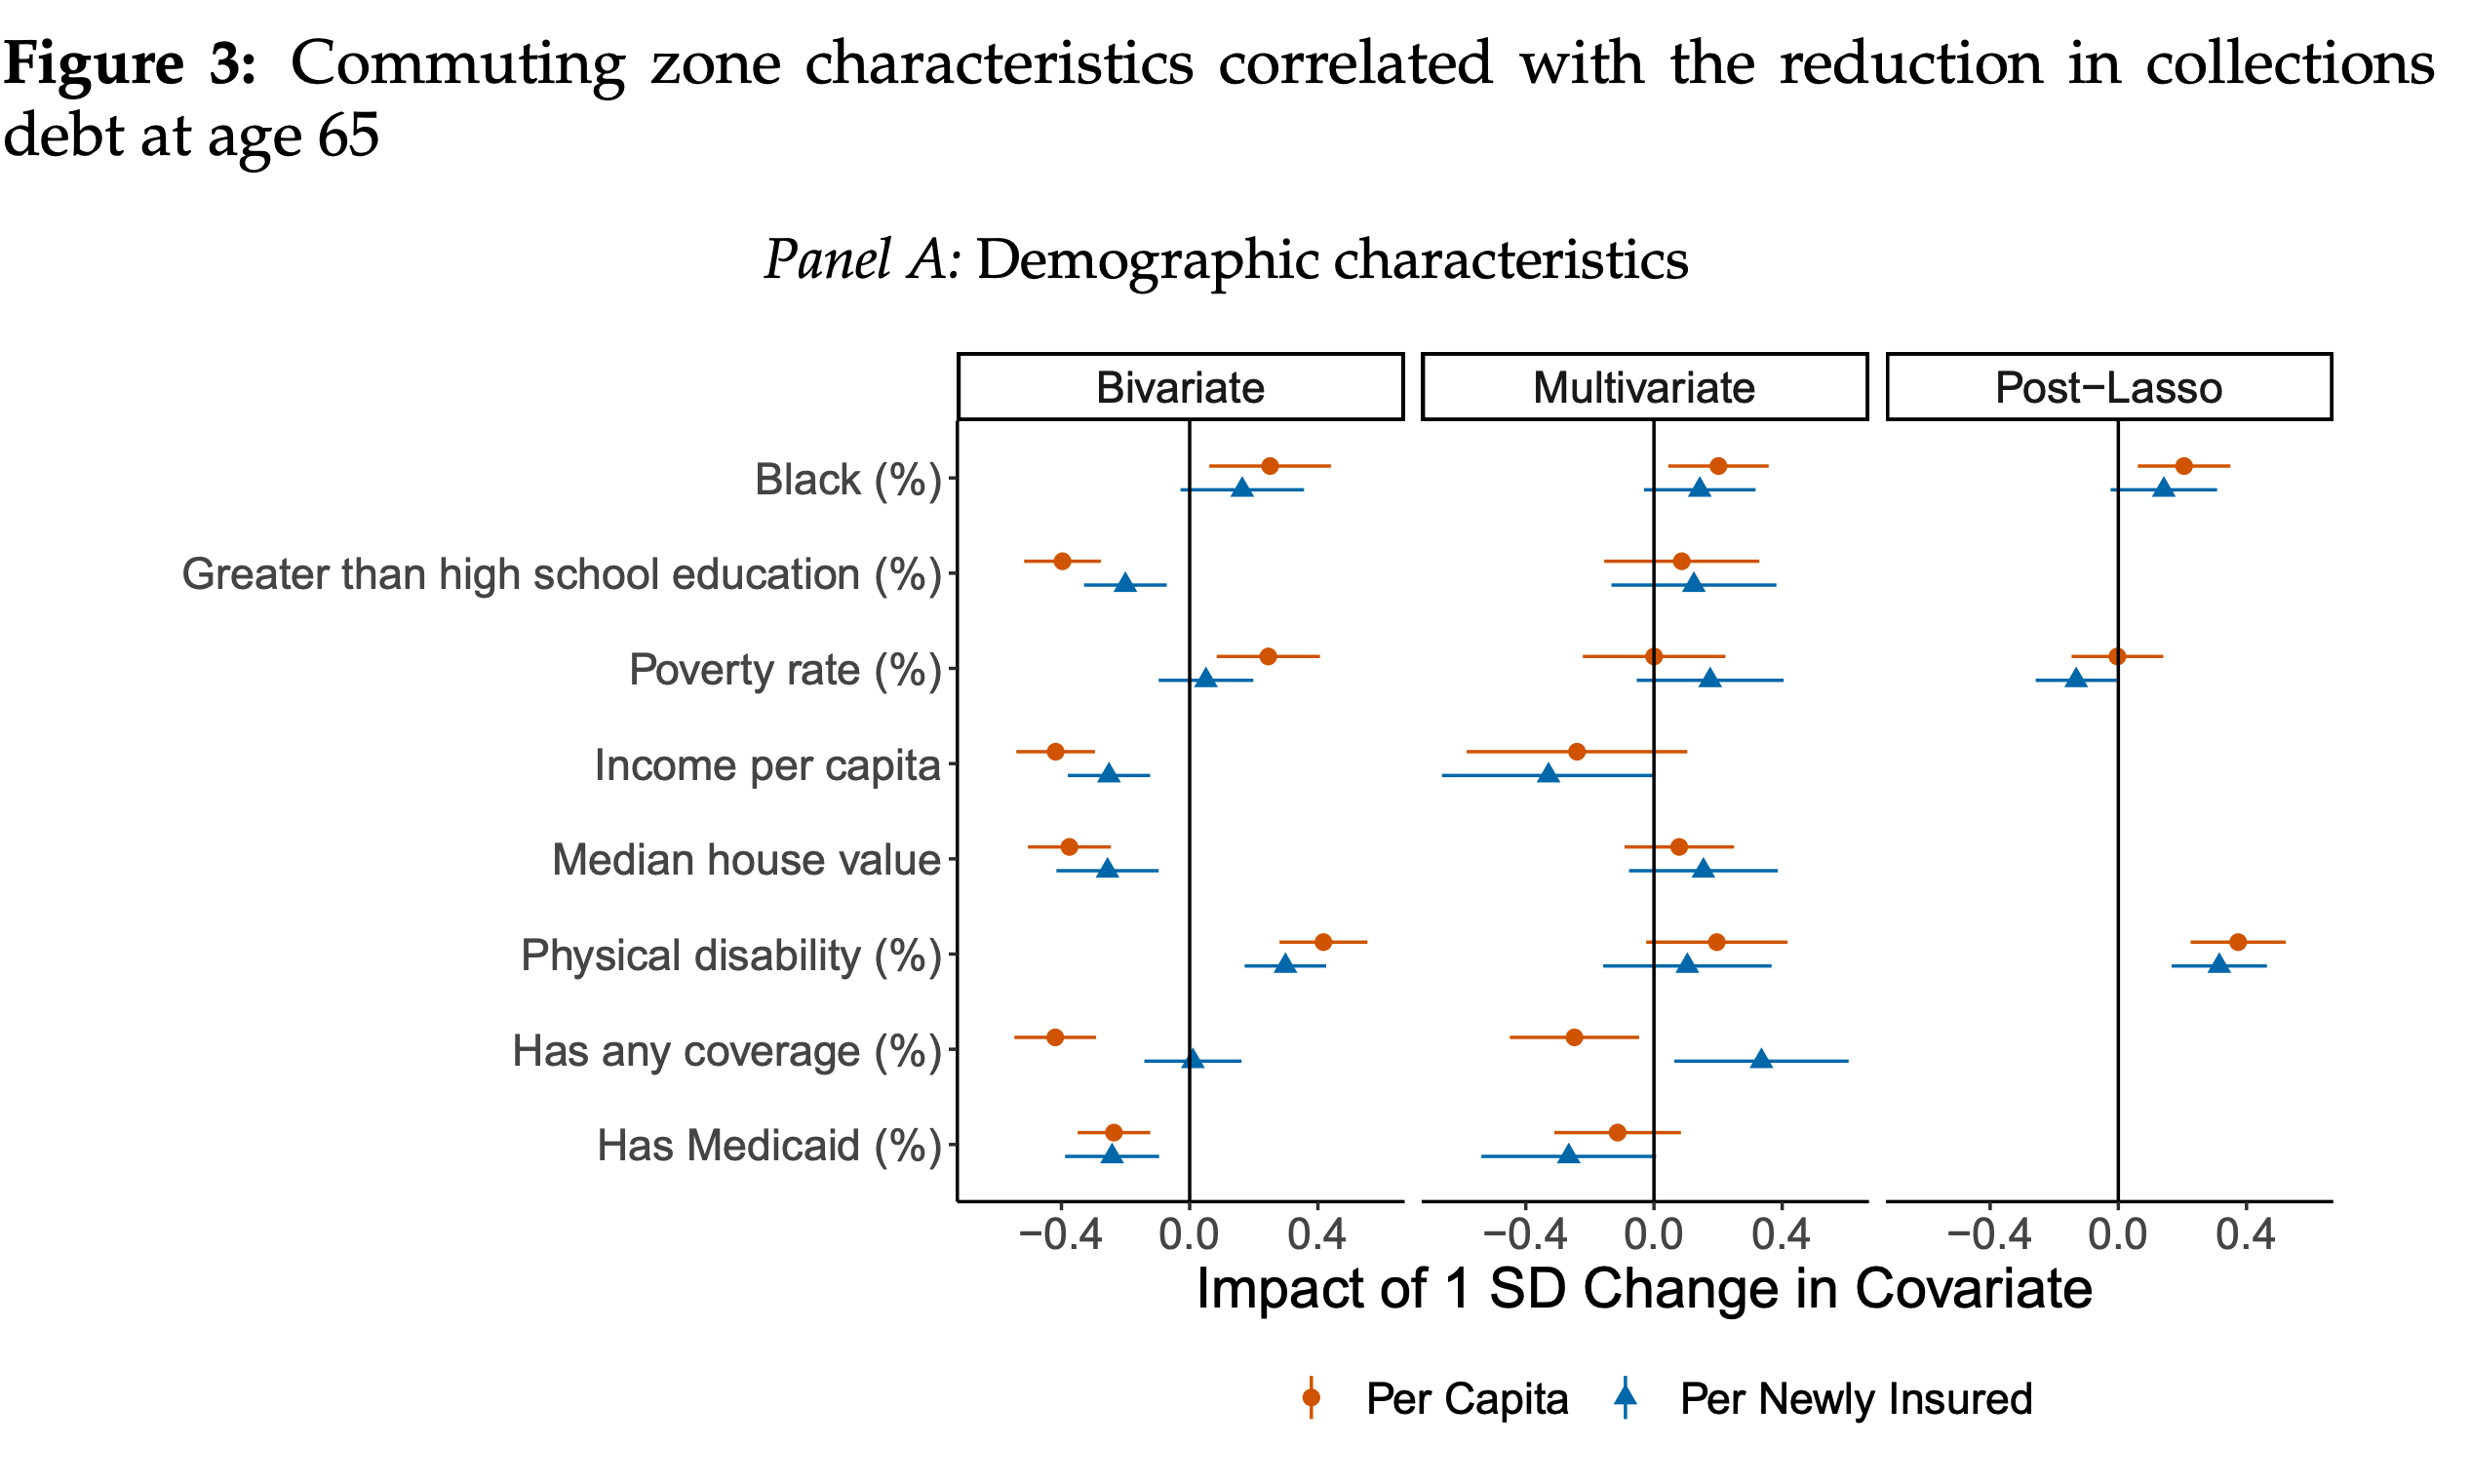
\includegraphics[width=\linewidth]{images/gpw_figure.png}
      }
    \only<3>{
        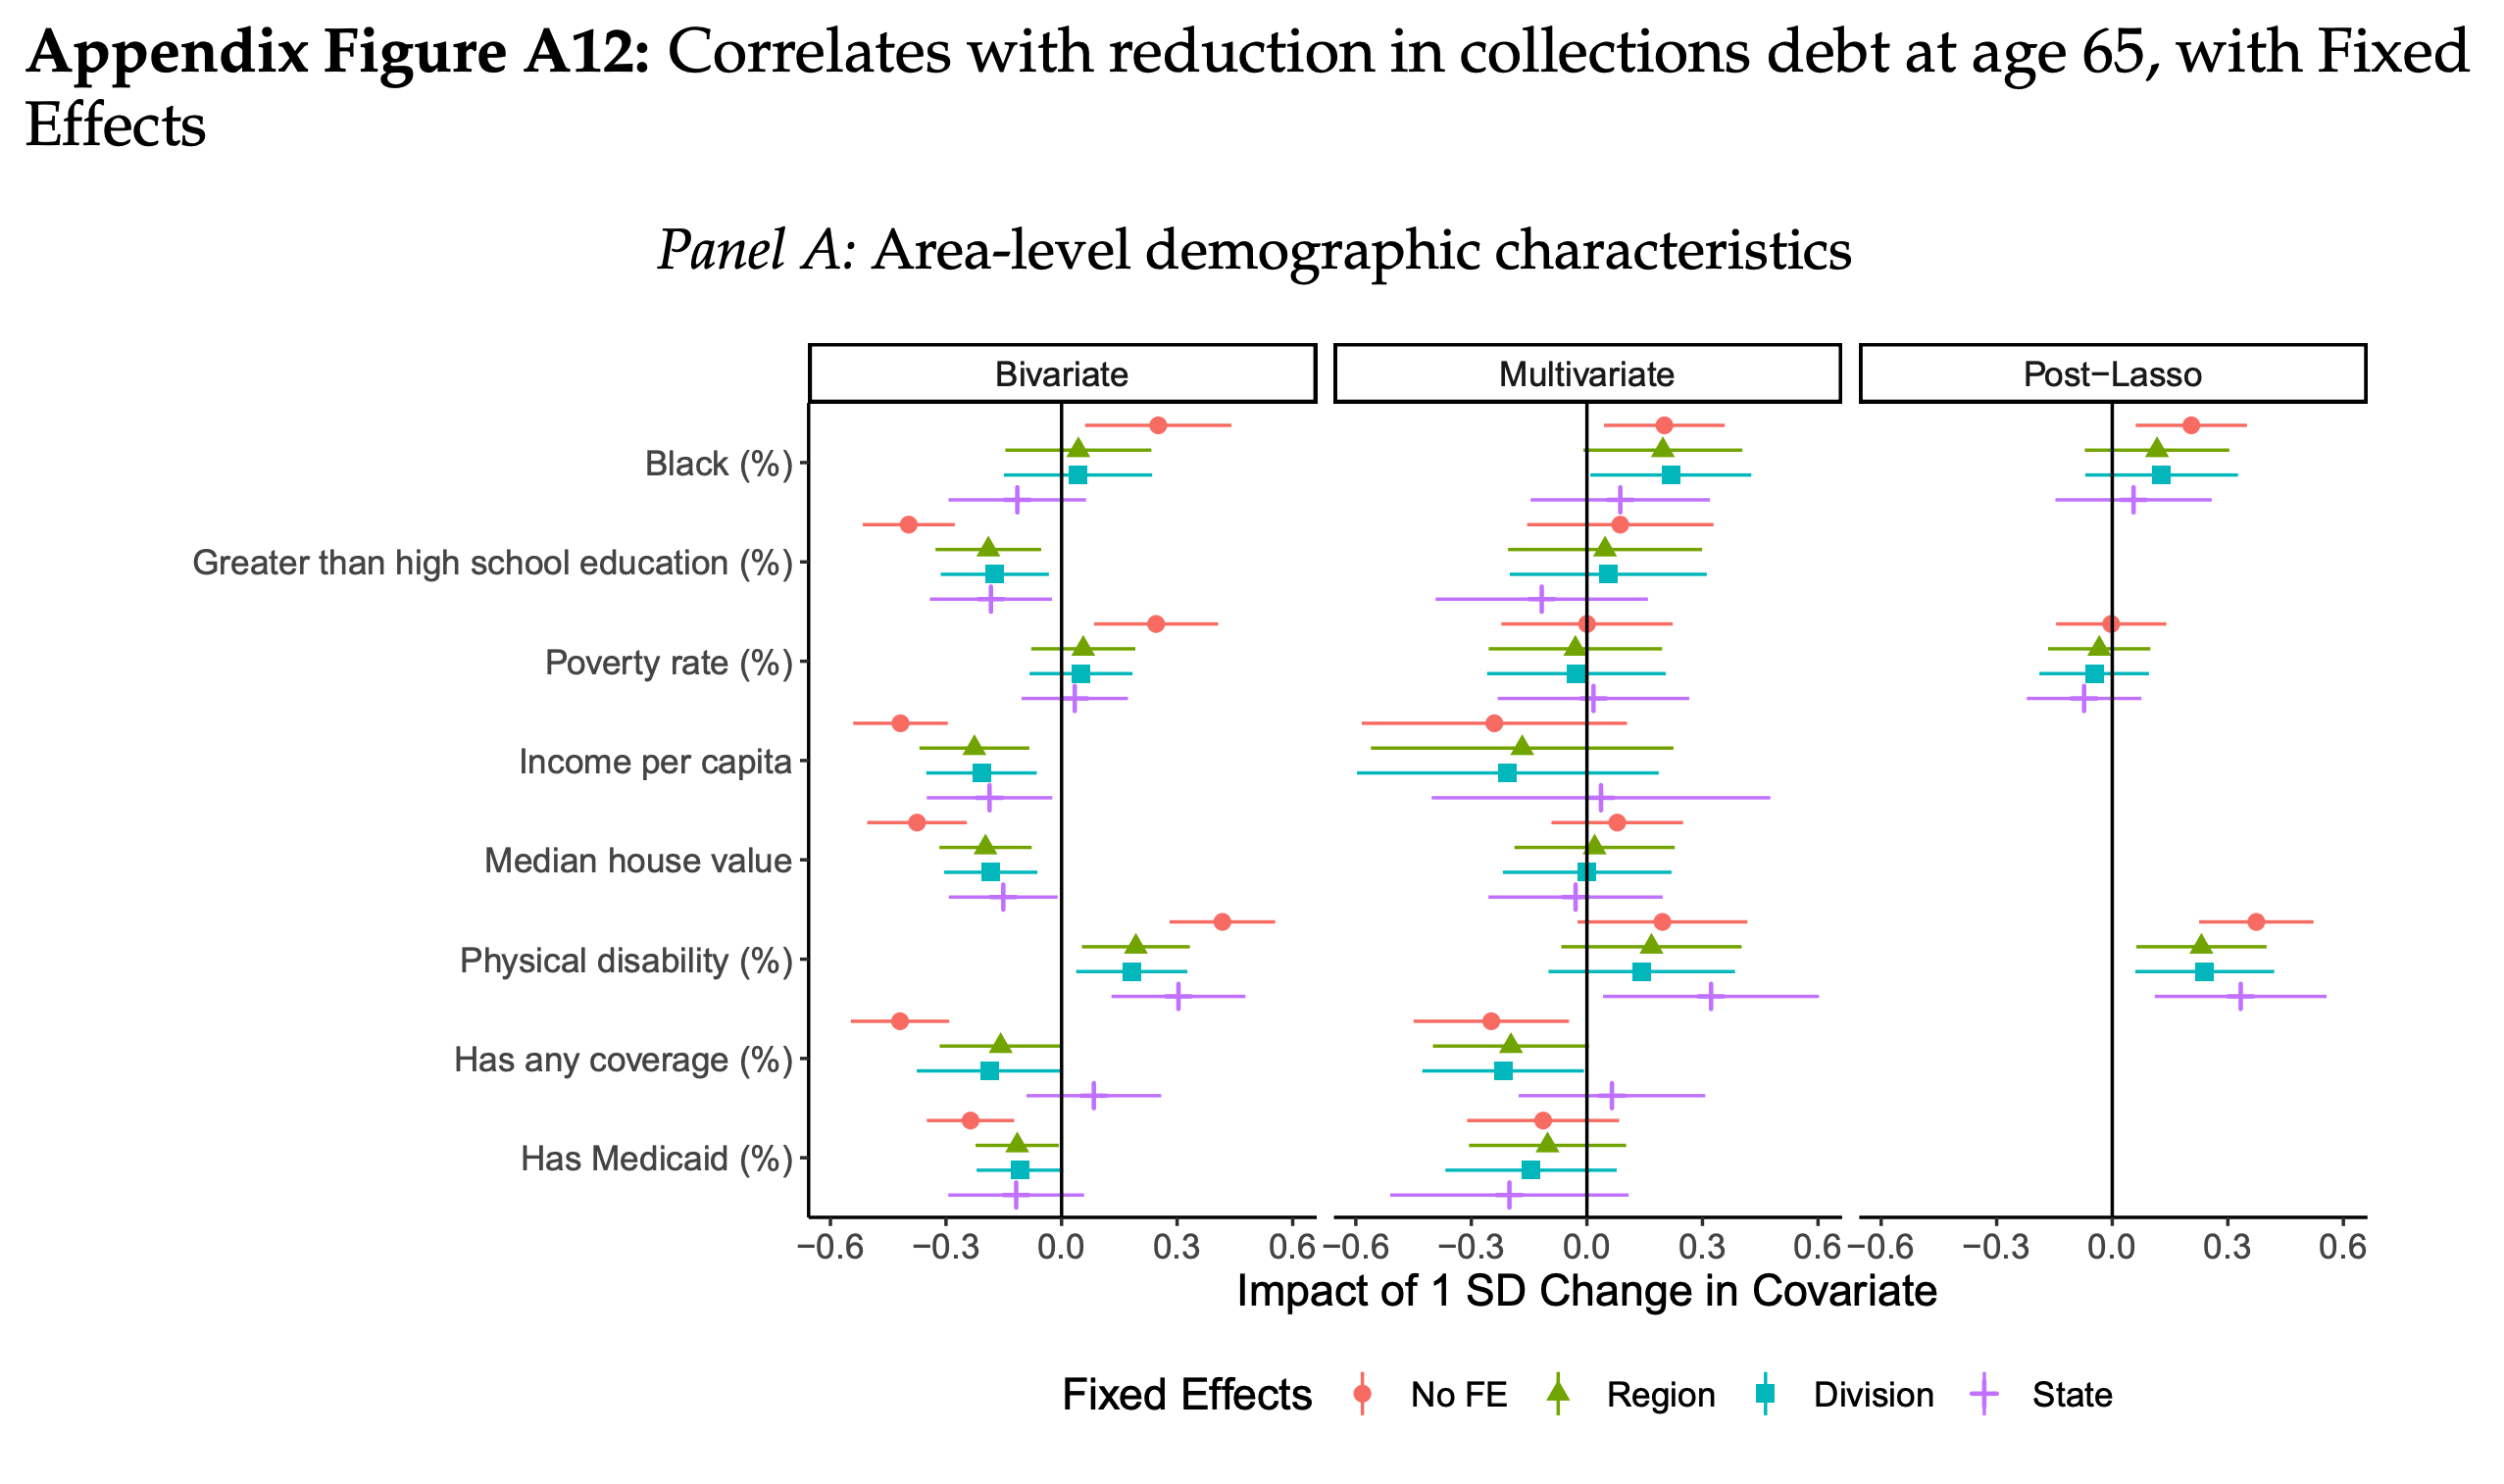
\includegraphics[width=\linewidth]{images/gpw_figure2.png}
      }
    \only<4>{
        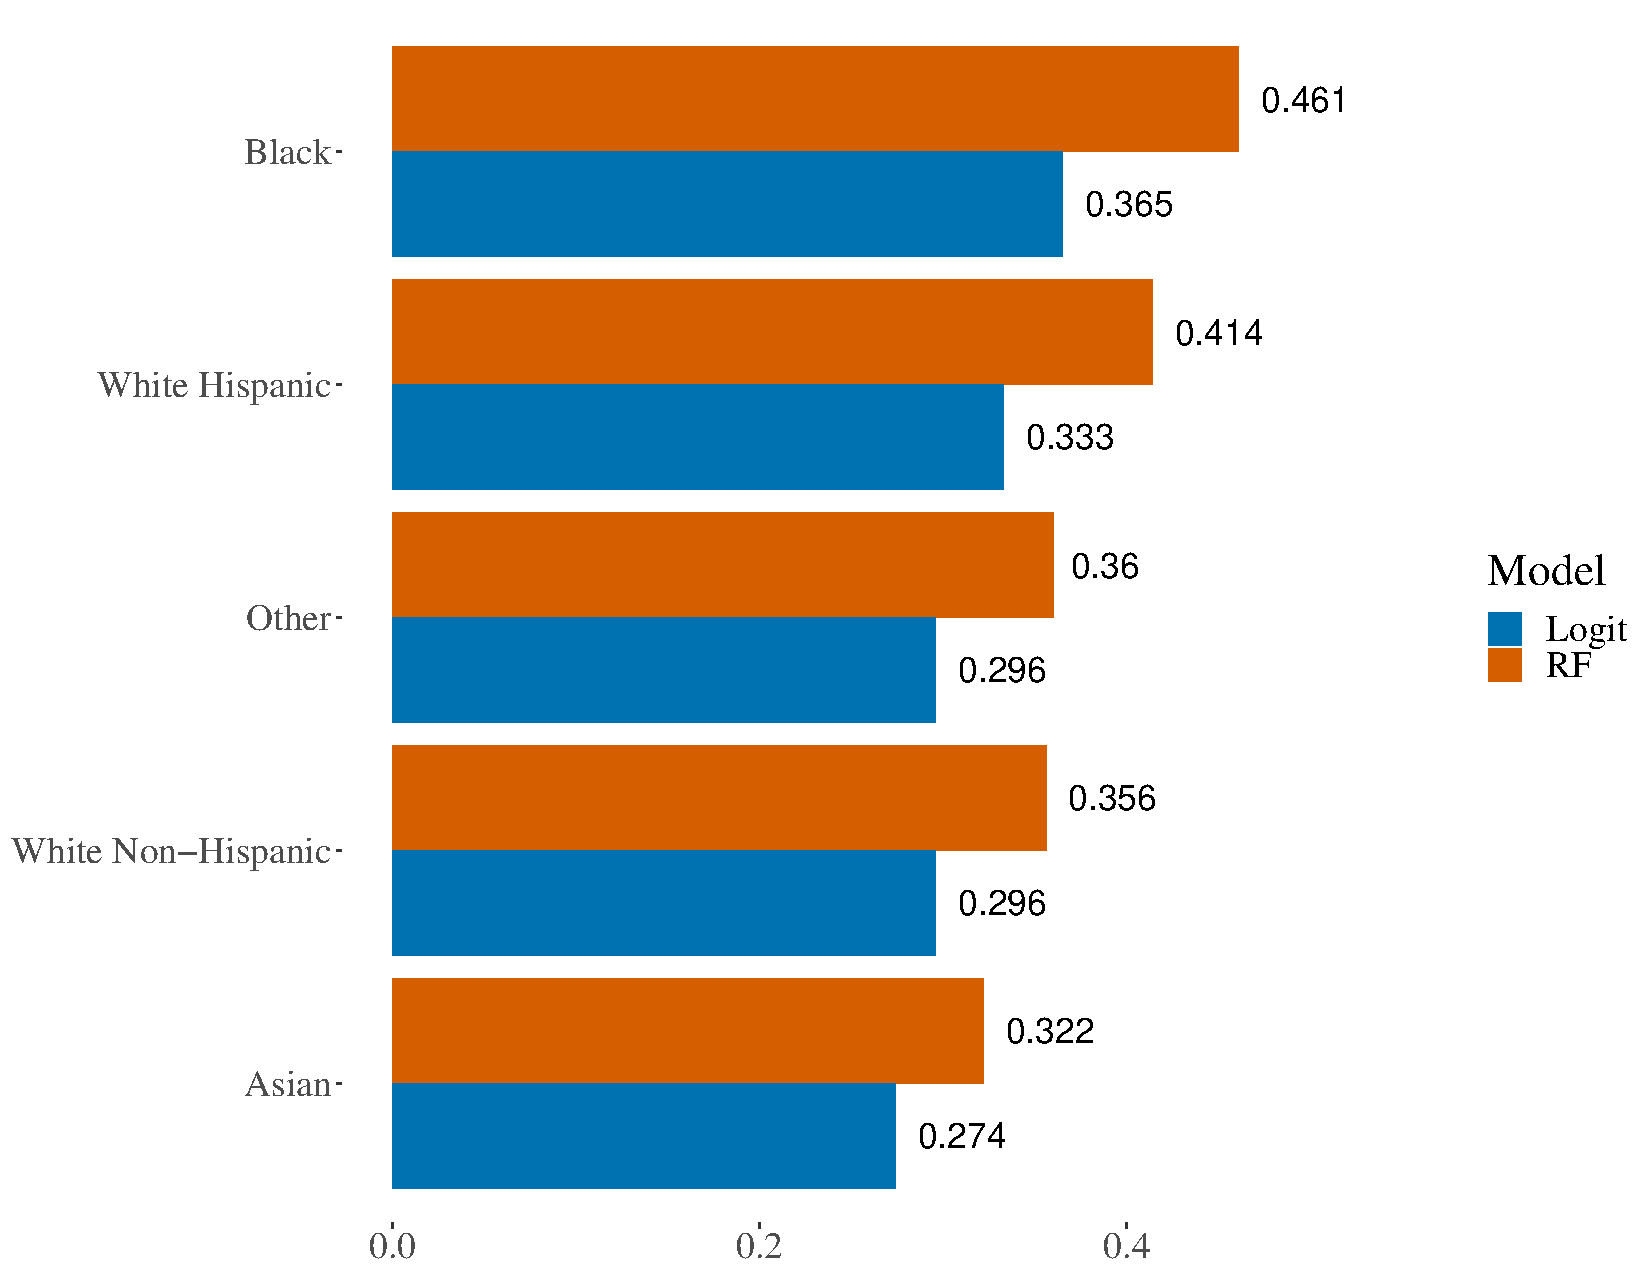
\includegraphics[width=\linewidth]{images/sato_sd_model.pdf}
      }
  \end{column}
\end{columns}
\end{frame}



\begin{frame}{2. Describable Goals}
  \begin{columns}[T] % align columns
    \begin{column}{.6\textwidth}
      \begin{wideitemize}
      \item When considering a figure, for most papers you want the
        result to be obvious
        \begin{itemize}
        \item Research papers' exhibits typically are not
          ``exploratory''
        \end{itemize}
      \item If it is not immediately obvious what the goal of an
        exhibit is, one of two things are likely occuring
        \begin{itemize}
        \item You have too much information, and the story you are telling is lost
        \item You have too little information or highlighting of the
          relevant piece that you're interested in
        \end{itemize}
      \item Jon Schwabish describes this as ``preattentive
        processing'' -- how do we emphasize certain pieces of a figure
        for the reader?
      \end{wideitemize}
  \end{column}%
  \hfill%
  \begin{column}{.4\textwidth}
  \end{column}
\end{columns}
\end{frame}


\begin{frame}{3. Craft not-ugly figures}
  \begin{columns}[T] % align columns
    \begin{column}{.6\textwidth}
      \begin{wideitemize}
      \item There is huge variation in how much researchers value figures
        \begin{itemize}
        \item I'm quite aware I fall on an extreme of that distribution
        \end{itemize}
      \item Nonetheless, there's almost no good reason to have \emph{bad} figures
      \item Avoiding this entails a small amount of work for big
        returns.  For this example, we could:
        \begin{enumerate}
        \item Fix the scheme (e.g. blue on white is ugly)
        \item Label our axes
        \item Make our color scheme clearer
        \item Thicken the line fit, and lighten the points 
        \end{enumerate}
      \end{wideitemize}
  \end{column}%
  \hfill%
  \begin{column}{.4\textwidth}
    \only<1>{    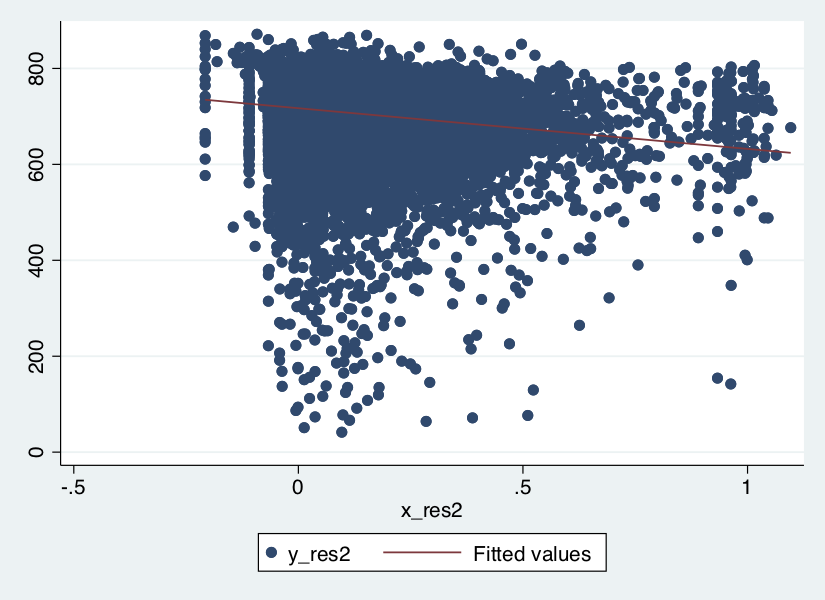
\includegraphics[width=\linewidth]{images/example_scatter_bad.png}
    }
    \only<2>{    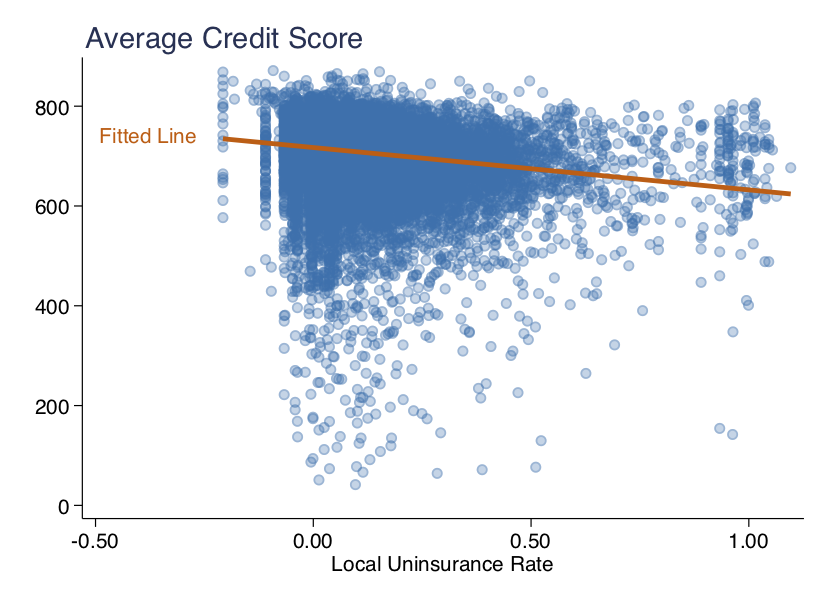
\includegraphics[width=\linewidth]{images/graph_fixed_up.png}
      }
  \end{column}
\end{columns}
\end{frame}

\begin{frame}{4. Do not mislead your readers}
  \begin{columns}[T] % align columns
    \begin{column}{.7\textwidth}
      \begin{wideitemize}
      \item Readers will percieve things in certain ways, and you can exploit that
        \begin{itemize}
        \item For good or for evil! Pick good.
        \end{itemize}
      \item Consider the following example (from my own work which I have since changed)
        \begin{itemize}
        \item In many event study settings, we plot the dynamic coefficients
        \item We typically have period by period data -- don't want to
          imply smoothness that isn't there
        \item My (updated) view: better to use pointwise caps, as the
          smooth lines imply something that is not true
        \end{itemize}
      \item Also important -- keep improving your graphs! All graphs
        can be improved, but you don't have to improve every graph.
      \end{wideitemize}
  \end{column}%
  \hfill%
  \begin{column}{.4\textwidth}
    \only<1>{    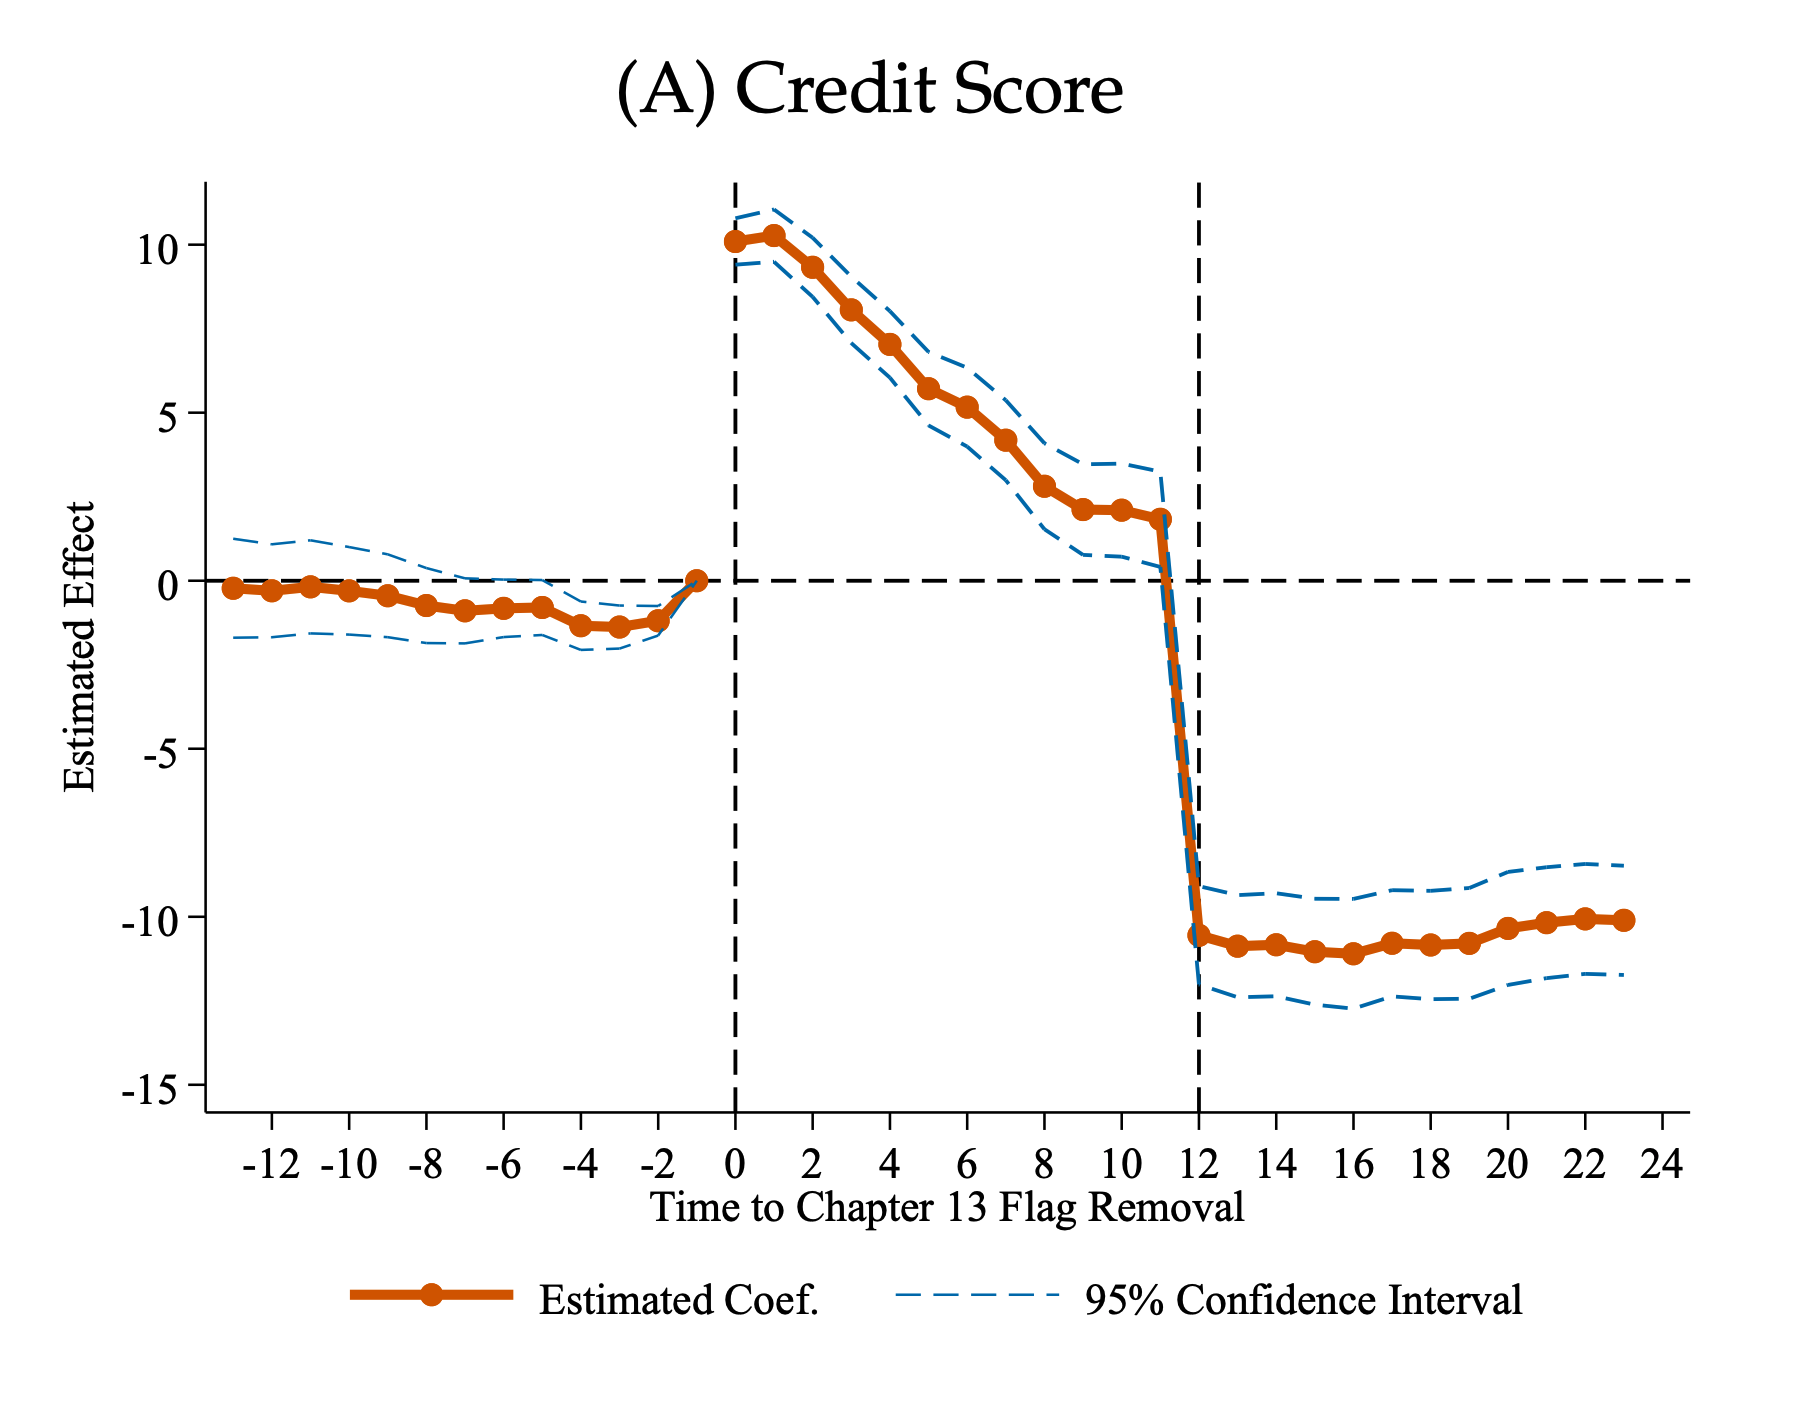
\includegraphics[width=\linewidth]{images/credit_score_bkflag.png}
      }
    \only<2>{    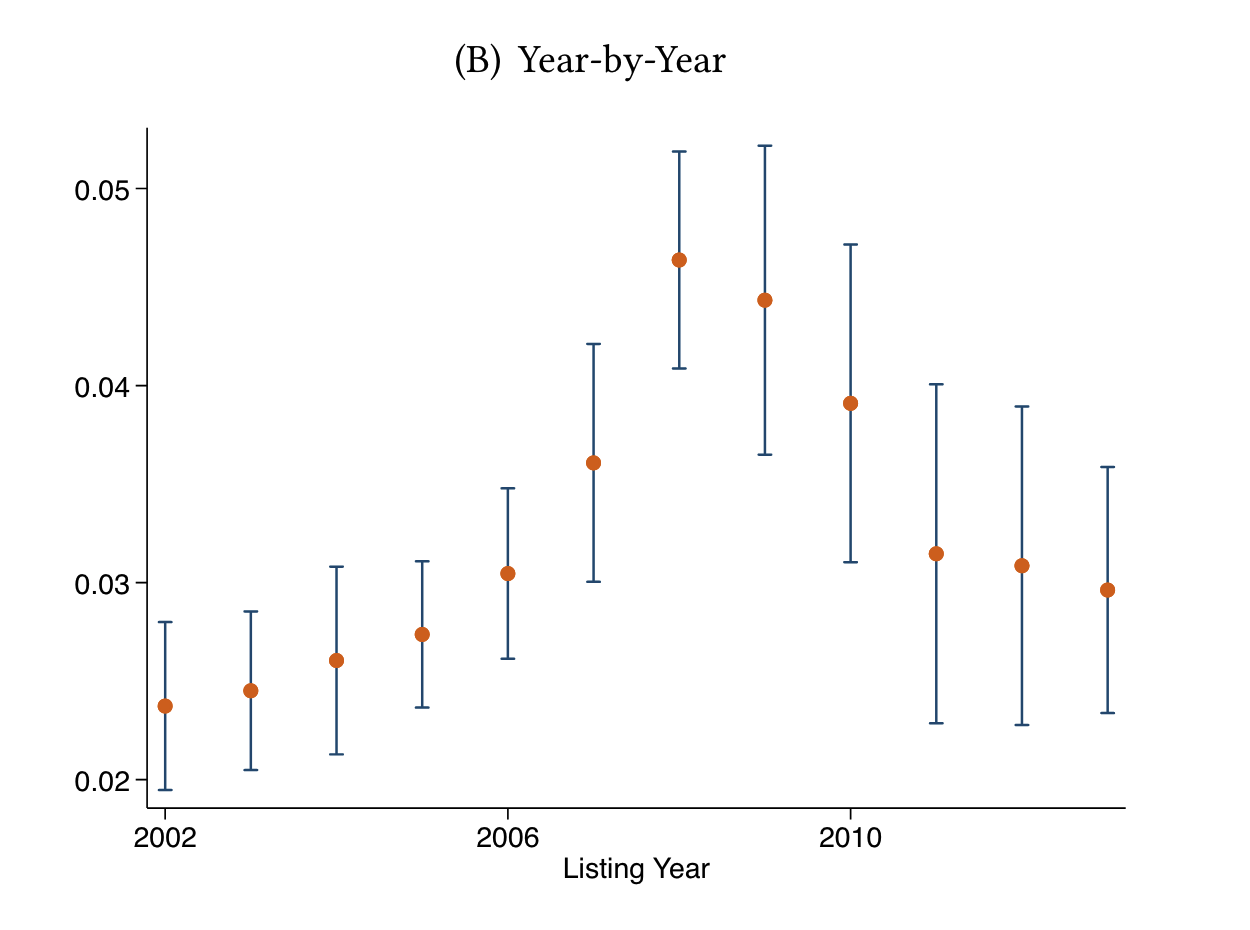
\includegraphics[width=\linewidth]{images/agent_effect_yearly.png}
      }
  \end{column}
\end{columns}
\end{frame}

\begin{frame}{Making good figures is hard}
  Some suggestions:
  \begin{wideitemize}
  \item Bar graphs are always good places to start. Make them
    horizontal (almost always) so that your labels are readable.
  \item Don't put confidence intervals on bar graphs. Use a point
    range plot instead
  \item Directly label on your figure as much as you can -- it makes
    it much easier for the reader to pay attention to what is going on
  \item Fix your units
    \begin{itemize}
    \item Round numbers, add commas, put dollar signs, put zero
      padding
    \end{itemize}
  \item Label your axes, but label your y-axis at the top of your
    graph rather than turned 90 degrees on the side
  \item Use gestalt principles to highlight things in your graphs:
    \begin{itemize}
    \item Shapes, thickness, saturation, color, size, markings,
      position, sharpness
    \end{itemize}
  \end{wideitemize}
  
\end{frame}

\begin{frame}{Making good figures is hard}
  \begin{columns}[T] % align columns
    \begin{column}{.6\textwidth}
  \begin{wideitemize}
  \item We are not the NYTimes -- we do not need to make insanely polished visualizations
  \item Most of our results will be relatively simple, but we will
    have a lot of versions of it that we need to convey
    \begin{itemize}
    \item Key: provide a polished way to provide a bite-sized piece of information
    \item Then, once the reader understands that, a large host of
      other information is also easily processed
    \item E.g., consider these figures from my paper
    \end{itemize}
  \item A lot going on, but in given panel, can break down into bite
    sized pieces
    \begin{itemize}
    \item Each subsequent result is then easily understood
    \end{itemize}
  \end{wideitemize}
  \end{column}%
  \hfill%
  \begin{column}{.4\textwidth}
    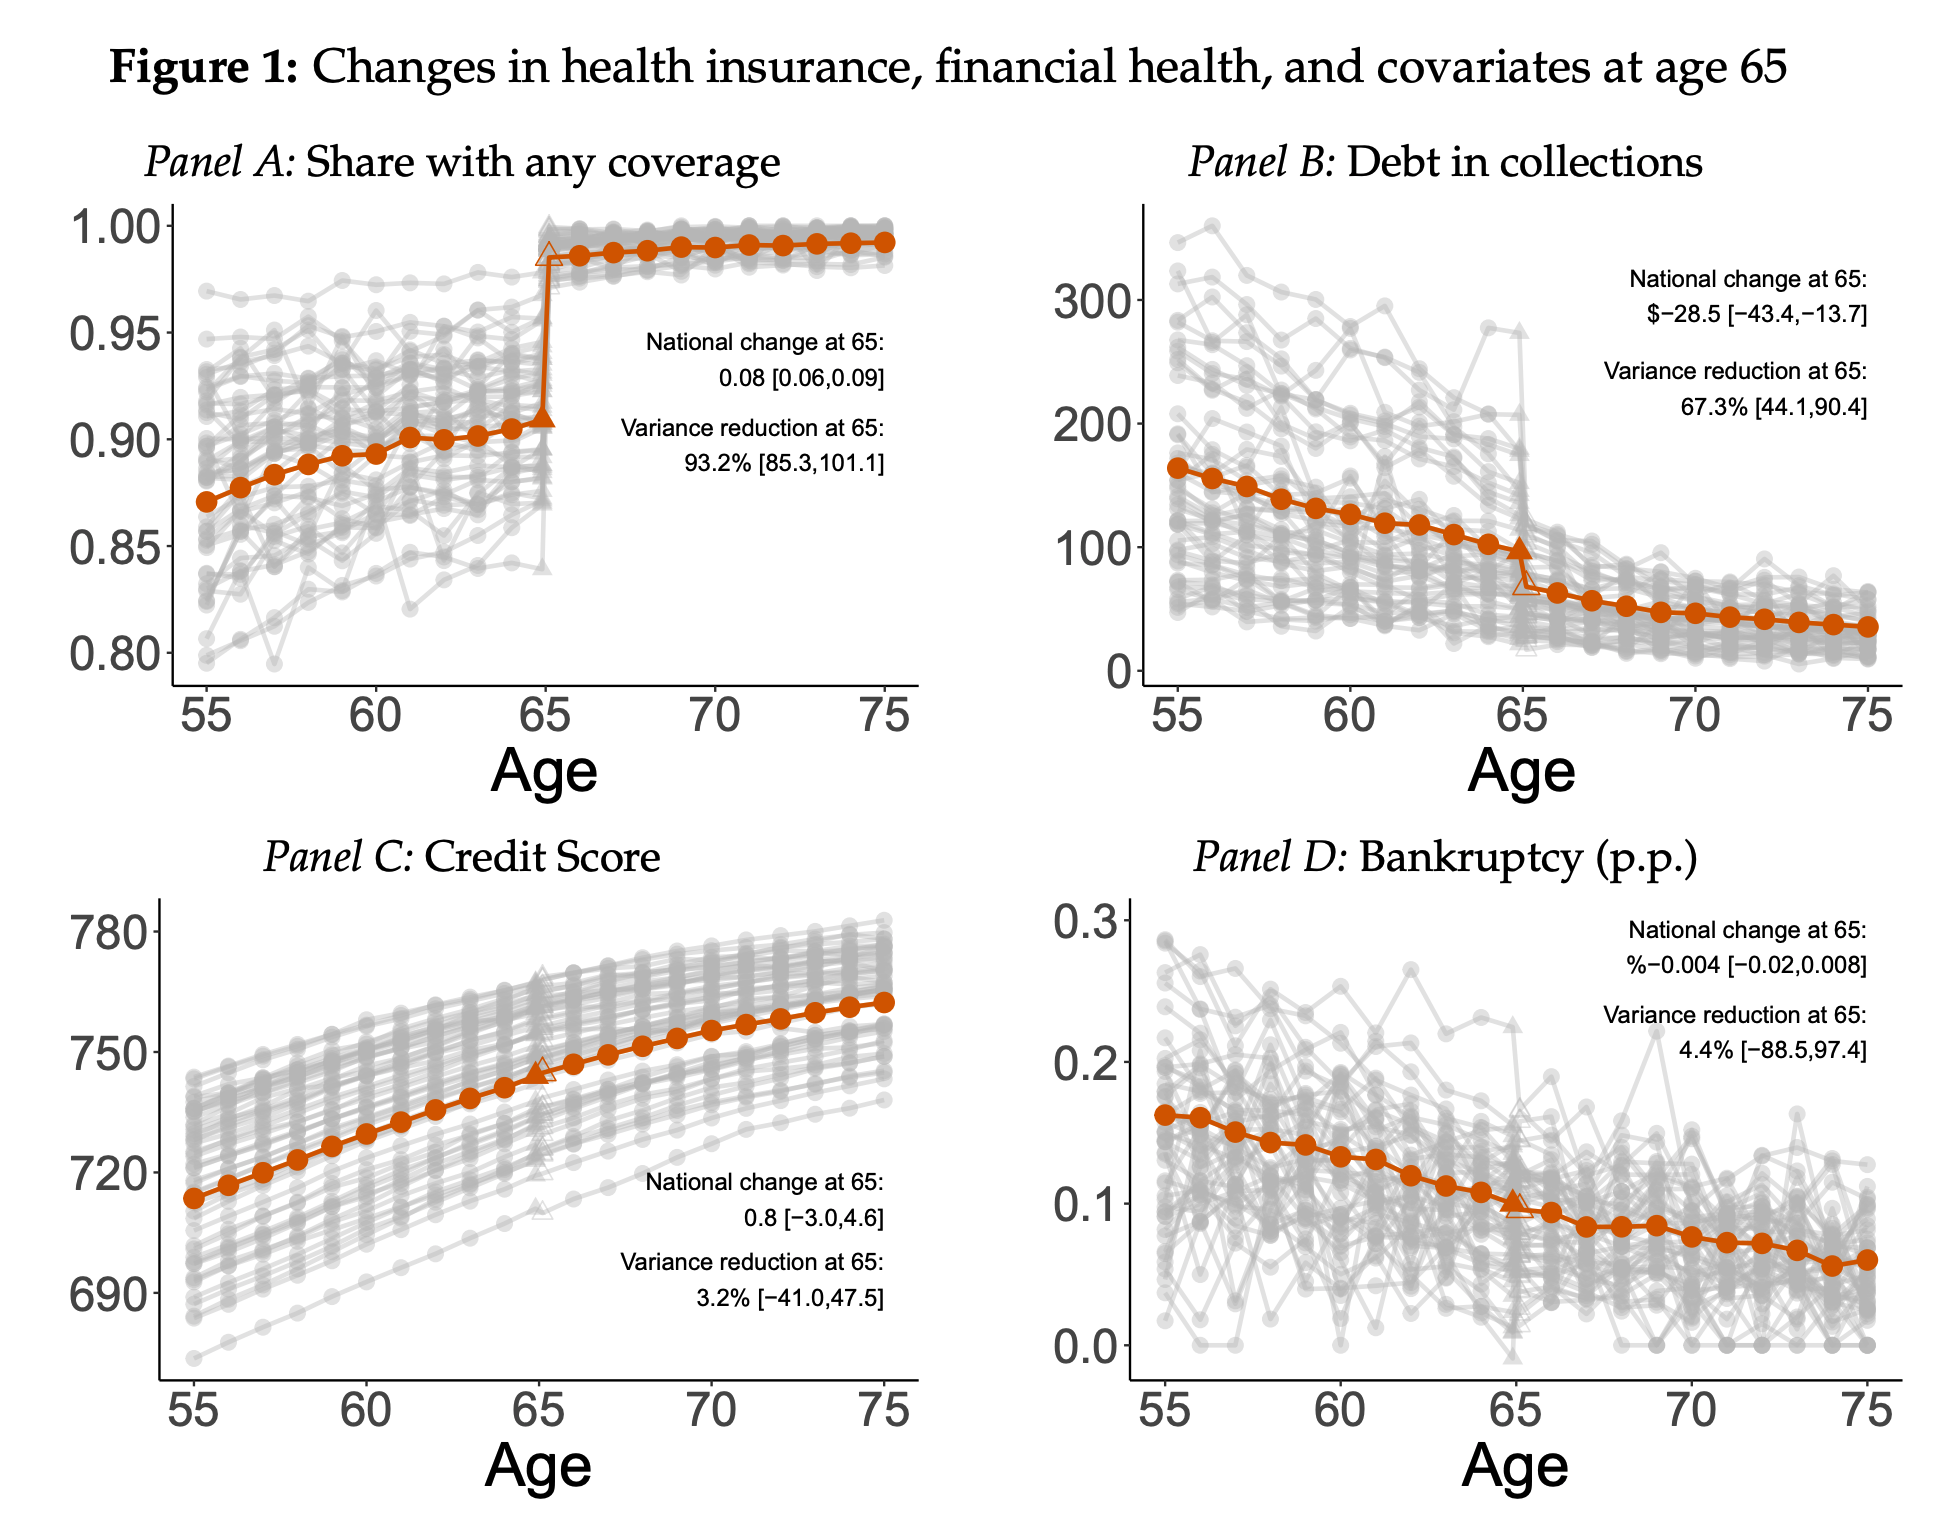
\includegraphics[width=\linewidth]{images/gpw_example.png}
  \end{column}
\end{columns}
\end{frame}


\end{document}